\documentclass[a4paper]{article}
\usepackage[top=2cm, bottom=2cm, left=1.5cm, right=1.5cm]{geometry}
\usepackage[german]{babel}
\usepackage[utf8]{inputenc}
\usepackage[T1]{fontenc}
\usepackage{eso-pic}
\usepackage{fontspec}   %%custom font
\usepackage{graphicx}   %%images
\setmainfont{[MahaloBrother.ttf]} %%costumfont
\usepackage{sectsty}    %% colored sections
\usepackage{datetime}
\usepackage{multicol}
\usepackage[usenames,dvipsnames]{color}
\usepackage{tikz}
\usetikzlibrary{matrix}
\usepackage{caption}
\usepackage{wrapfig}
\usepackage{float}
\usepackage[most]{tcolorbox}
%%%%
%%% add lines to page  %%%
\usepackage{tikzpagenodes}
\usepackage{lipsum}
\usepackage{background}
%%%%





\usepackage{hyperref}
\hypersetup{
    colorlinks=true,
    linkcolor=blue,
    filecolor=magenta,      
    urlcolor=cyan,
    pdftitle={Overleaf Example},
    pdfpagemode=FullScreen,
    }


\usepackage{fancyhdr}

\pagestyle{fancy}
\fancyhf{}
\lhead{ITB16-LF2}
\fancyhead[CE,CO]{LF2-Klausur}
\fancyfoot[CE,CO]{\Large{LF2-Klausur Vorbereitung}}
\rhead{\today}
\rfoot{Seite \thepage}
\lfoot{\href{mailto://ammohammed@schueler.berufskolleg.de}{Amer M. Mohammed}}


\usepackage{smartdiagram}
\usepackage{\dtklogos}

\usepackage{listings}
\usepackage[table,xcdraw]{xcolor}

\hypersetup{
    colorlinks=true,
    linkcolor=blue,
    filecolor=magenta,      
    urlcolor=cyan,
    pdftitle={Overleaf Example},
    pdfpagemode=FullScreen,
    }
    
\usepackage{amsmath}



\usepackage{xfakebold}

\newcommand{\fbseries}{\unskip\setBold\aftergroup\unsetBold\aftergroup\ignorespaces}
\makeatletter
\newcommand{\setBoldness}[1]{\def\fake@bold{#1}}
\makeatother
\setBoldness{0.4}%
\chapterfont{\color{blue}}  % sets colour of chapters
\sectionfont{\color{cyan}}  % sets colour of sections
\subsectionfont{\color{violet}}
\subsubsectionfont{\color{purple}}


%% colors 

\definecolor{notepadrule}{RGB}{217,244,244}
\definecolor{codegreen}{rgb}{0,0.6,0}
\definecolor{codegray}{rgb}{0.5,0.5,0.5}
\definecolor{codepurple}{rgb}{0.58,0,0.82}
\definecolor{backcolour}{rgb}{0.95,0.95,0.92}



\tikzset{ 
    table/.style={
        matrix of nodes,
        row sep=-\pgflinewidth,
        column sep=-\pgflinewidth,
        nodes={
            rectangle,
            draw=blue,
            align=left
        },
        minimum height=1.5em,
        text depth=0.5ex,
        text height=2ex,
        nodes in empty cells,
%%
        every even row/.style={
            nodes={fill=purple!20}
        },
        column 1/.style={
            nodes={text width=2em,font=\bfseries}
        },
        row 1/.style={
            nodes={
                fill=cyan,
                text=white,
                font=\bfseries
            }
        }
    }
}


\lstdefinestyle{mystyle}{
    backgroundcolor=\color{backcolour},   
    commentstyle=\color{codegreen},
    keywordstyle=\color{magenta},
    numberstyle=\tiny\color{codegray},
    stringstyle=\color{codepurple},
    basicstyle=\ttfamily\footnotesize,
    breakatwhitespace=false,         
    breaklines=true,                 
    captionpos=b,                    
    keepspaces=true,                 
    numbers=left,                    
    numbersep=5pt,                  
    showspaces=false,                
    showstringspaces=false,
    showtabs=false,                  
    tabsize=2
}

\lstset{style=mystyle}





\begin{document}

    \begin{titlepage}
        \AddToShipoutPictureBG*{
\includegraphics[width=\paperwidth,height=\paperheight]{media/bglf2}}

\begin{figure}[!htb]
    \centering
    
\includegraphics[width=7cm]{logo-3}\label{fig:figure}
\end{figure}

\begin{center}
    \color{white}\Huge{\colorbox{BurntOrange}{\fbseries  LF2}}
    \vspace{5mm}
    \\ \color{black}\small{\colorbox{white}{\fbseries Berufskolleg Hilden des Kreises Mettmann}}
    \vspace{5mm}
    \\  \color{white}\Huge{\colorbox{BurntOrange}{Amer Malik Mohammed}}
\end{center}

\vspace{15mm}
\begin{center}
    {\color{white}\LARGE{\textbf{\vspace{30mm}} \colorbox{BurntOrange}{ITB16}\\\vspace{5mm}\colorbox{BurntOrange}{Lehrer: Herr Epping}}}
\end{center}



\color{white}\centering\large\colorbox{BurntOrange}{letzte Bearbeitung}

\color{white}\centering\large\colorbox{BurntOrange}{\today\hspace{0.2cm}\currenttime}

    \end{titlepage}

%%% lines to page %%%%
    \backgroundsetup{
contents={%   
  \begin{tikzpicture}
    \foreach \fila in {0,...,44}
    {
      \draw [line width=1pt,color=notepadrule] 
      (current page.west|-0,-\fila*16pt) -- ++(\paperwidth,0);
    }
    \draw[overlay,red!70!black,line width=1pt]
      ([xshift=-1pt]current page text area.west|-current page.north) --  
      ([xshift=-1pt]current page text area.west|-current page.south);
  \end{tikzpicture}%
},
scale=1,
angle=0,
opacity=1
}
%%% end lines to page %%%

    \section{Vorwort}\label{sec:einführung}
    \paragraph{Dieses Dokument wurde am \today\hspace{0.2cm}\currenttime\hspace{0.2cm} fertiggestellt. Bitte zögern Sie nicht, \href{https://github.com/amermmohammed/LF2_Klausurvorbereitung}{dieses Repository} zu klonen, um Informationen hinzuzufügen, zu ändern, zu optimieren oder zu korrigieren, wenn Informationen bearbeitet werden müssen. Andernfalls können Sie jederzeit prüfen, ob es eine neue Version des Dokuments gibt. Ich plane jedoch, jede neue Version dieses Dokuments bis zum Sonntag, den 03.04.22 Nachmittag in unserer WhatsApp-Gruppe ITB16 zu teilen.}
    \paragraph{\\\\\\\\\\\\\\\\\\\\}
    \begin{center}
        
        \color{red}
        \colorbox{yellow}{Haftungsausschluss}
    \end{center}
    \paragraph{\color{white} \centering\colorbox{red}{Die Verwendung dieses Dokuments liegt in Ihrer Verantwortung. Ich habe mein Bestes getan, um die darin} \\\colorbox{red}{enthaltenen Informationen zusammenzufassen. Die Verwendung der Informationen zur } \\\hspace{1cm}\colorbox{red}{Beantwortung einer Frage in einem Test oder einer Prüfung usw. liegt in Ihrer eigenen Verantwortung.}}
    \begin{center}
        \color{red}
        \colorbox{yellow}{Amer Malik Mohammed}
    \end{center}
    \newpage
    \tableofcontents
    \newpage
    
    \section{Kühlsysteme}\label{sec:kuehlsysteme}

    \subsection{\color{red}Nenne PC-Komponenten, die gekühlt werden müssen?}\label{subsec:nenne-pc-komponenten-die-gekühlt-werden-müssen?}

    \paragraph{\color{codegreen}Alle Komponenten, die Strom verbrauchen}
    \begin{itemize}
        \color{magenta}
        \item CPU
        \item Motherboard
        \item Grafikkarte
        \item Netzteil
        \item Arbeitsspeicher
        \item Festplatte
    \end{itemize}

    \subsection{\color{red}beschreibe die Funktionsweise von unterschiedlichen Kühlarten}\label{subsec:beschreibe-die-funktionsweise-von-unterschiedlichen-kühlarten}

    \paragraph{\color{codegreen}Luftstroms}
    \begin{itemize}
        \color{magenta}
        \item Kalte Luft ins Gehäuse
        \item Warme Luft raus
    \end{itemize}

    \paragraph{\color{codegreen}Wasserstrom}
    \begin{itemize}
        \color{magenta}
        \item  Kaltes Wasser zu der Hardware gepumpt
        \item Warmes Wasser wird am Radiator vom Lüfter gekühlt
    \end{itemize}

    \subsection{\color{red}nenne Vor- und Nachteile der unterschiedlichen Kühlarten}\label{subsec:nenne-vor--und-nachteile-der-unterschiedlichen-kühlarten}

    \subsubsection{\color{codegreen}Luftstroms}
    \begin{center}
        \begin{tabular}{cclll}
            \cline{1-2}
            \multicolumn{1}{|c|}{\textbf{Vorteile}}                          & \multicolumn{1}{c|}{\textbf{Nachteile}}                      &  &  &  \\ \cline{1-2}
            \multicolumn{1}{|c|}{{\color[HTML]{32CB00} Preis}}               & \multicolumn{1}{c|}{{\color[HTML]{F56B00} Weniger Leistung}} &  &  &  \\ \cline{1-2}
            \multicolumn{1}{|c|}{{\color[HTML]{32CB00} Leichter einzubauen}} & \multicolumn{1}{c|}{{\color[HTML]{F56B00} Staubfänger}}      &  &  &  \\ \cline{1-2}
            \multicolumn{1}{l}{}                                             & \multicolumn{1}{l}{}                                         & & &
        \end{tabular}
    \end{center}

    \subsubsection{\color{codegreen}Wasserkühlung}
    \begin{center}
        \begin{tabular}{|c|clll}
            \cline{1-2}
            \textbf{Vorteile}                                            & \multicolumn{1}{c|}{\textbf{Nachteile}}                          & & & \\ \cline{1-2}
            {\color[HTML]{32CB00} Mehr Leistung}                         & \multicolumn{1}{c|}{{\color[HTML]{F56B00} Komplizierter Einbau}} &  &  &  \\ \cline{1-2}
            {\color[HTML]{32CB00} Leiser}                                & \multicolumn{1}{c|}{{\color[HTML]{F56B00} Teurer}}               &  &  &  \\ \cline{1-2}
            \multicolumn{1}{|l|}{{\color[HTML]{32CB00} CPU Übertaktung}} & \multicolumn{1}{l}{}                                             &  &  &  \\ \cline{1-1}
        \end{tabular}
    \end{center}

    \section{Ergonomie}\label{sec:ergonomie}

    \subsection{\color{red}Nenne Größen der Temperatur, der Lautstärke und der Luftfeuchtigkeit für ein gutes Raumklima}\label{subsec:nenne-größen-der-temperatur-der-lautstärke-und-der-luftfeuchtigkeit-für-ein-gutes-raumklima}
    \begin{itemize}
        \color{magenta}
        \item Angenehme Raumtemperatur 21 bis 22° Celsius
        \item Im Sommer Obergrenze von 26° Celsius
        \item relative Luftfeuchtigkeit sollte 50 – 65 \% betragen
        \item Ideal sind Fenster zum Lüften und regelmäßige Stoßlüftung.
        \item Zum Schutz vor Sommerhitze sind Sonnenschutzvorrichtungen notwendig.
        \item \color[HTML]{F56B00} Lärm
        \begin{itemize}
            \item Schallpegel in einem Büro: höchstens 30 – 40 dB
            \item vorwiegend Geistigen Tätigkeiten: max.
            55 dB
            \item einfachen oder mechanischen Büroarbeiten: max.
            60 dB
        \end{itemize}
    \end{itemize}

    \subsection{\color{red}Beschreibe die Anforderungen an den Arbeitsplatz für eine gesunde Sitzhaltung}\label{subsec:beschreibe-die-anforderungen-an-den-arbeitsplatz-für-eine-gesunde-sitzhaltung}
    \begin{itemize}
        \color{magenta}
        \item Bildschirmoberkante nicht oberhalb
        der waagerechten Blicklinie
        \item Geeigneten Sehabstand zum
        Monitor schaffen.
        \item Tastatur ca.
        10--15 cm von
        der Tischkante entfernt parallel
        aufstellen.
        \item Maus nicht mit gestrecktem Arm bedienen, Mauspad ggf.
        mit Handballenauflage.
    \end{itemize}

    \subsection{\color{red}Beschreibe, wie der Arbeitsplatz im Raum (zur Fensterseite) angeordnet sein sollte}\label{subsec:beschreibe-wie-der-arbeitsplatz-im-raum-(zur-fensterseite)-angeordnet-sein-sollte}
    \begin{itemize}
        \color{magenta}
        \item Aufstellung des Tisches, so dass
        Blickrichtung parallel zum Fenster
        verläuft.
        \item Monitor gerade vor sich aufstellen,
        keine verdrehten Körperhaltungen
        \item • bei mehreren Fenstern parallel
        zur tageslichtintensitäten Fensterseite
        sitzen.
    \end{itemize}

    \subsection{\color{red}Erkläre, Vorteile einer ergonomischen Maus und Tastatur}\label{subsec:erkläre-vorteile-einer-ergonomischen-maus-und-tastatur}

    \paragraph{\color{codegreen} Eine \color{red} ergonomische Tastatur \color{codegreen} hat eine ergonomische Form und ist häufig noch zusätzlich verstellbar, damit Sie in einer natürlichen, ergonomischen Haltung am Computer arbeiten können. Beschwerden an Fingern, Handgelenk, Unterarm und Schulter können so verhindert oder behoben werden.}

    \paragraph{\color{codegreen} Eine \color{red}ergonomische Maus \color{codegreen} ist vertikal aufgebaut, wodurch Elle und Speichel parallel übereinander stehen und somit Sehnen, Muskeln und Nerven so wenig wie möglich belastet werden.}

    \section{Prozessor}\label{sec:prozessor}
    \begin{wrapfigure}{r}{.3\textwidth}
        \centering
        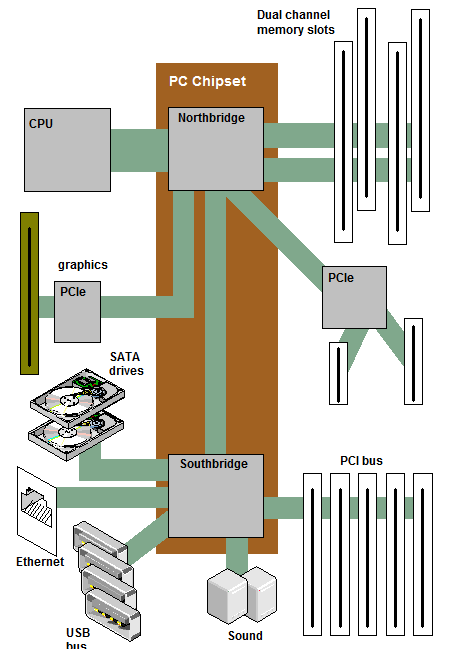
\includegraphics[scale=.2]{media/sb-nb}
        \captionsetup{labelformat=empty}
        \caption{Northbridge/Southbridge-Chipsatz\\\color{red}\small{Der Northbridge-Teil des Chipsatzes steuert die Hochgeschwindigkeitskanäle, während die Southbridge die Geräte mit niedrigerer Geschwindigkeit steuert.}}
        \label{fig:bridges}
    \end{wrapfigure}

    \subsection{\color{red}Beschreibe die Aufgaben der North- und Southbridge eines Chipsatzes}\label{subsec:beschreibe-die-aufgaben-der-north--und-southbridge-eines-chipsatzes}

    \subsubsection{\color{codegreen}Northbridge}

    \paragraph{\color{codegreen}Der Hochgeschwindigkeitsteil einer gemeinsamen Chipsatzarchitektur in einem Computer. Die Northbridge ist der Controller, der die CPU über den Frontside-Bus (FSB) mit dem Speicher verbindet. Es verbindet auch Peripheriegeräte über Hochgeschwindigkeitskanäle wie PCI Express. Die Northbridge kann einen Anzeigecontroller enthalten, wodurch die Notwendigkeit einer separaten Grafikkarte entfällt.}

    \paragraph{\color{red}Northbridge Verbindet die CPU mit:}
    \begin{itemize}
        \color{magenta}
        \item RAM
        \item Eingebaute Grafik
        \item PCI-Express (PCIe)
    \end{itemize}

    \subsubsection{\color{codegreen}Southbridge}

    \paragraph{\color{codegreen}Der Southbridge-Controller verarbeitet die restlichen I/O, einschließlich PCI-Bus, parallele und Serial ATA-Laufwerke (IDE), USB, FireWire, serielle und parallele Anschlüsse und Audioanschlüsse. Frühere Chipsätze unterstützten den ISA-Bus in der Southbridge. Beginnend mit den 8xx-Chipsätzen von Intel wurden Northbridge und Southbridge in Memory Controller und I/O Controller geändert}

    \paragraph{\color{red}Southbridge Verbindet die CPU mit:}
    \begin{itemize}
        \color{magenta}
        \item SATA-Laufwerke
        \item USB-Bus
        \item Eingebautes Audio
    \end{itemize}

    \subsection{\color{red}Beschreibe die Aufbau eines modernen Chipsatzes mit einem Platform Controller Hub bzw. Fusion Controller Hub (ohne Northbridge)}\label{subsec:beschreibe-die-aufbau-eines-modernen-chipsatzes-mit-einem-platform-controller-hub-bzw.-fusion-controller-hub-(ohne-northbridge)}

    \subsubsection{\color{codegreen}Platform Controller Hub (PCH)}
    \paragraph{\color{codegreen}Im Jahr 2008 wurde mit der Einführung des Chipsatzes der Intel 5-Serie die Northbridge/Southbridge-Architektur durch die Platform Controller Hub (PCH)-Architektur ersetzt. In dieser Architektur wird die Southbridge-Funktionalität vom PCH-Chip verwaltet, der über das DMI direkt mit der CPU verbunden ist.\newline
    Die meisten Northbridge-Funktionen wurden in die CPU integriert, während der PCH die restlichen Funktionen zusätzlich zu den traditionellen Rollen der Southbridge übernahm. In der PCH-Architektur sind die RAM- und PCIe-Datenpfade direkt mit der CPU verbunden. Beispiele für x86-Architekturen, bei denen die Northbridge in die CPU integriert ist, sind Intels Sandy Bridge und AMDs Fusion.\newline}

    \begin{center}
        \begin{figure}[H]
            \centering
            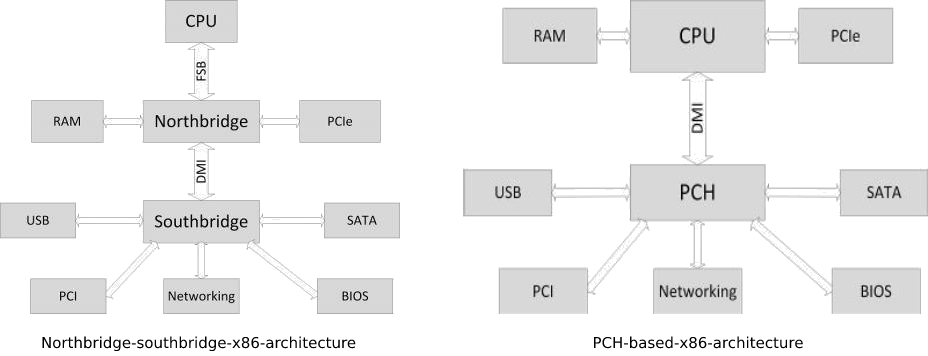
\includegraphics[height=5cm]{media/PCHVSN-S-bridge}
            \captionsetup{label-format=empty}
            \caption{north- south bridge vs PCH architecture}\label{fig:architecture}
        \end{figure}
    \end{center}

    \subsubsection{\color{codegreen}Fusion controller hubs (FCH)}

    \paragraph{\color{codegreen}{\fbseries Die Fusion Controller Hubs ähneln in ihrer Funktion dem Platform Controller Hub (PCH) von Intel. } Für AMD APU-Modelle von 2011 bis 2016. AMD vermarktet seine Chipsätze als Fusion Controller Hubs (FCH) und implementiert sie 2017 zusammen mit der Veröffentlichung der Zen-Architektur in seiner gesamten Produktpalette. Davor verwendeten nur APUs FCHs, während ihre anderen CPUs noch eine Northbridge und Southbridge verwendeten.}

    \subsection{\color{red}Beschreibe die Begriffe ALU, FPU und FLOPS}\label{subsec:beschreibe-die-begriffe-alu-fpu-und-flops}

    \subsubsection{\color{codegreen}arithmetic logic unit (ALU)}

    \paragraph{\color{codegreen} Eine arithmetisch-logische Einheit ist ein elektronisches Rechenwerk, welches in Prozessoren zum Einsatz kommt. { \fbseries Die ALU berechnet arithmetische und logische Funktionen.}}

    \paragraph{\color{red}Mögliche Rechenoperationen}
    \begin{itemize}
        \color{magenta}
        \item Addition
        \item Subtraktion (Negativ-Addition)
        \item Vergleich
        \item Multiplikation
        \item Division
    \end{itemize}

    \paragraph{\color{red}Mögliche logische Verknüpfungen}
    \begin{itemize}
        \color{magenta}
        \item AND, OR, XOR
        \item Bitverschiebung
    \end{itemize}

    \subsubsection{\color{codegreen}Floating Point Unit (FPU)}

    \paragraph{\color{codegreen} Eine Gleitkommaeinheit (FPU) ist ein Teil eines Computersystems, das speziell dafür ausgelegt ist, Operationen mit Gleitkommazahlen auszuführen. Typische Operationen sind Addition, Subtraktion, Multiplikation, Division und Quadratwurzel. Einige FPUs können auch verschiedene transzendente Funktionen wie exponentielle oder trigonometrische Berechnungen ausführen, aber die Genauigkeit kann sehr gering sein, sodass einige Systeme es vorziehen, diese Funktionen in Software zu berechnen.}

    \subsubsection{\color{codegreen}Floating Point Operations Per Second (FLOPS)}

    \paragraph{\color{codegreen} Die Anzahl der Gleitkommaoperationen, die eine Recheneinheit (Prozessor oder gesamtes Rechnersystem) pro Sekunde ausführen kann. FLOPS werden als Maßeinheit benutzt, um die Rechenleistung von Systemen zu beschreiben..}

    \subsection{\color{red}Erläutere die technische Angabe der Fertigungstechnik(z.B.7nm)}\label{subsec:erläutere-die-technische-angabe-der-fertigungstechnik(z.b.7nm)}

    \paragraph{\color{codegreen}7 Nanometer bezieht sich auf die Größe der beteiligten Transistoren. Je kleiner der Transistor ist, desto mehr passt auf ein Stück Silizium und desto leistungsfähiger und komplexer können die aus diesen Transistoren aufgebauten Komponenten sein.}

    \paragraph{\large{TO DO}}

    \subsection{\color{red}Erkläre den Nutzen und den Aufbau von Cache-Speicher}\label{subsec:erkläre-den-nutzen-und-den-aufbau-von-cache-speicher}

    \paragraph{\color{codegreen} Der Cache-Speicher oder Cache Memory ist eine chipbasierte Computerkomponente, die das Abrufen von Daten aus dem Speicher des Computers effizienter macht. Er dient als temporärer Speicherbereich, aus dem der Prozessor des Computers Daten leicht abrufen kann. Dieser temporäre Speicherbereich, der als Cache bezeichnet wird, steht dem Prozessor leichter und schneller zur Verfügung als der Hauptarbeitsspeicher (Main Memory) des Computers, normalerweise eine Form von DRAM.}
    \subsubsection{\color{codegreen}Arten von Cache Memory}

    \paragraph{\color{red}Cache-Speicher ist schnell und teuer. Traditionell wird er in „Ebenen“ (Levels) kategorisiert, die seine Nähe und Zugänglichkeit zum Mikroprozessor beschreiben. Es gibt drei allgemeine Cache-Ebenen:}
    \begin{itemize}
        \color{magenta}
        \item {\fbseries Der L1-Cache } oder primäre Cache ist extrem schnell, aber relativ klein und wird normalerweise als CPU-Cache in den Prozessor-Chip eingebettet.
        \item {\fbseries Der L2-Cache } oder sekundäre Cache ist oft umfangreicher als der L1-Cache.
        Der L2-Cache kann in die CPU eingebettet sein, oder er kann sich auf einem separaten Chip oder Ko-Prozessor befinden und über einen alternativen Hochgeschwindigkeits-Systembus verfügen, der den Cache und die CPU verbindet.
        Auf diese Weise wird er nicht durch den Verkehr auf dem Hauptsystembus verlangsamt.
        \item {\fbseries Der Cache } der Ebene 3 (L3) ist ein spezialisierter Arbeitsspeicher, der entwickelt wurde, um die Leistung von L1 und L2 zu verbessern.
        L1 oder L2 können wesentlich schneller sein als L3, obwohl L3 normalerweise doppelt so schnell wie DRAM ist.
        Bei Mehrkernprozessoren kann jeder Kern (Core) über einen dedizierten L1- und L2-Cache verfügen, aber sie können sich einen L3-Cache teilen.
        Wenn ein L3-Cache auf eine Anweisung verweist, wird er normalerweise auf eine höhere Cache-Ebene angehoben.
    \end{itemize}

    \subsection{\color{red}Beschreibe die Programmiersprache Assembler}\label{subsec:beschreibe-die-programmiersprache-assembler}
    \paragraph{\color{codegreen} Assemblersprache ist jede Low-Level-Programmiersprache, in der eine sehr starke Entsprechung zwischen den Anweisungen in der Sprache und den Maschinencodeanweisungen der Architektur besteht.
    Assemblercode wird durch ein Dienstprogramm, das als Assembler bezeichnet wird, in ausführbaren Maschinencode umgewandelt. }
    
    \section{Monitore}\label{sec:monitore}

    \subsection{\color{red}Unterscheide die Panelarten TN, VA, IPS anhand von technischen Eigenschaften voneinander}\label{subsec:unterscheide-die-panelarten-tn-va-ips-anhand-von-technischen-eigenschaften-voneinander}
    \paragraph{\color{codegreen} Bei Flüssigkristall Monitor strahlt Licht durch rote, grüne und blaue Farbfilter. Die Flüssigkristalle lassen mal mehr, mal weniger dieses Licht durch und mischen so die Farben zusammen.\\
    Bei \color{red}{\fbseries TN-Panels }\color{codegreen} wechseln die Kristalle die Ausrichtung von horizontal auf vertikal. Bei \color{red}{\fbseries AV-Panels }\color{codegreen} genau umgekerht. Bei \color{red}{\fbseries IPS-Panels }\color{codegreen} drehen sich die Kristalle auf gleicher Ebene um 90 Grad.}
    \begin{center}
        \begin{figure}[H]
            \centering
            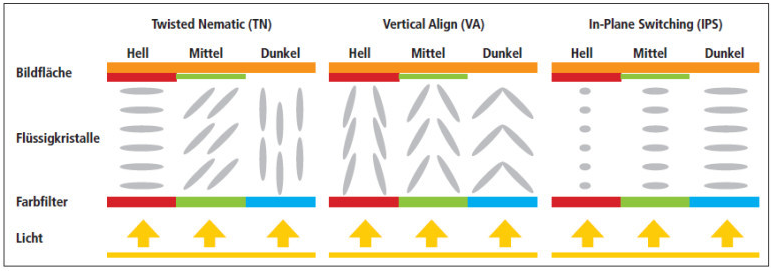
\includegraphics[height=5cm]{media/panals}
            \captionsetup{labelformat=empty}
            \caption{TN vs VA vs IPS}
            \label{fig:panals}
        \end{figure}
    \end{center}

    \subsection{\color{red}Erkläre, wie ein Pixel aufgebaut ist?}\label{subsec:erkläre-wie-ein-pixel-aufgebaut-ist?}

    \paragraph{\color{codegreen} Ein Pixel ist aus mehreren Subpixeln aufgebaut, die auf Monitoren und anderen Displays in Rot, Grün und Blau (RGB) wiedergegeben werden. Je nach Zusammensetzung dieser drei Farben entsteht ein bestimmter Farbton, der in Kombination mit meist Millionen anderer Bildpunkte das Gesamtbild ergibt.}

    \subsection{\color{red}Beschreibe die LCD- und OLED-Technik mit einfachen Worten}\label{subsec:beschreibe-die-lcd--und-oled-technik-mit-einfachen-worten}
    \begin{multicols}{2}
        \subsubsection{\color{codegreen}LCD-Bildschirm}
        \begin{itemize}
            \color{magenta}
            \item Beim LCD-Bildschirm werden Flüssigkristalle eingesetzt.
            Jeder dieser Kristalle stellt einen Bildpunkt, also ein Pixel, dar.
            \item Hinter den Flüssigkristallen befindet sich die Hintergrundbeleuchtung.
            Entweder durch LEDs, die aus den Ecken heraus leuchten oder durch Leuchtstoffröhren direkt hinter den Kristallen.
            \item Die Kristalle können einzeln ausgerichtet werden, so dass sie weniger oder mehr Licht durchlassen und die jeweilige Farbe wiedergeben.
        \end{itemize}

        \subsubsection{\color{codegreen}OLED-Bildschirm}
        \begin{itemize}
            \color{magenta}
            \item Der OLED-Bildschirm benötigt keine Hintergrundbeleuchtung.
            Stattdessen leuchtet jedes OLED für sich, jeder Bildpunkt ist also eine Lichtquelle.
            \item Das funktioniert mit zwei Elektroden, von denen eine transparent ist.
            Zwischen den beiden Elektroden befinden sich verschiedene organische Halbleiterschichten.
            \item Wird Strom durch die Elektroden geschickt, leuchten die Halbleiterschichten.
            Die Stromstärke reguliert die Helligkeit.
        \end{itemize}
    \end{multicols}
    \subsection{\color{red}Erkläre, technische Angaben zu einem Monitor (Bildwiederholungsrate, Auflösung, Pixeldichte,
        Größe (Zoll), Seitenverhältnis)}\label{subsec:erkläre-technische-angaben-zu-einem-monitor-(bildwiederholungsrate-auflösung-pixeldichte
    --------größe-(zoll)-seitenverhältnis)}

    \subsubsection{\color{codegreen}Bildwiederholungsrate (Bildwiederholfrequenz)}

    \paragraph{\color{codegreen} Die Bildwiederholfrequenz besagt, wie oft sich ein Vorgang pro Sekunde wiederholt. Ein 50-Hertz-Fernseher zeigt Bilder fünfzig Mal pro Sekunde, ein 100-Hertz-Gerät hundert Mal und so weiter.}

    \subsubsection{\color{codegreen}Auflösung}

    \paragraph{\color{codegreen} Die Auflösung eines Bildes wird in der Regel in „ppi“ (pixels per inch) angegeben und beschreibt, wie viele Pixel (digitale Bildpunkte) auf der Länge von einem inch/Zoll (2.54 cm) vorhanden sind.}

    \subsubsection{\color{codegreen}Pixeldichte}

    \paragraph{\color{codegreen} Die Pixeldichte von Displays ist ein Maß für den Grad des Auflösungsvermögens, wobei der Wert üblicherweise in dpi ausgedrückt wird. Dpi steht für „Punkte pro Zoll“ („Dots per Inch“, nicht pro Quadratzoll). Ein Zoll entspricht 2,54 Zentimeter.}

    \subsubsection{\color{codegreen}Größe (Zoll)}

    \paragraph{\color{codegreen} Ein Zoll ist etwas länger, als zweieinhalb Zentimeter, genau gilt: 1" = 2,54 cm. Das internationale Zoll wird als übliches Längenmaß vor allem noch in den USA verwendet sowie für festgelegte Größenangaben in der Technik.}

    \subsubsection{\color{codegreen}Seitenverhältnis}

    \paragraph{\color{codegreen} Unter Seitenverhältnis im weiteren Sinne versteht man das Verhältnis von mindestens zwei unterschiedlich langen Seiten eines Polygons. Meistens wird damit das Verhältnis der Breite eines Rechtecks zu seiner Höhe angegeben. Ein Quadrat hat das Seitenverhältnis 1:1.}
    \begin{center}
        \begin{figure}[H]
            \centering
            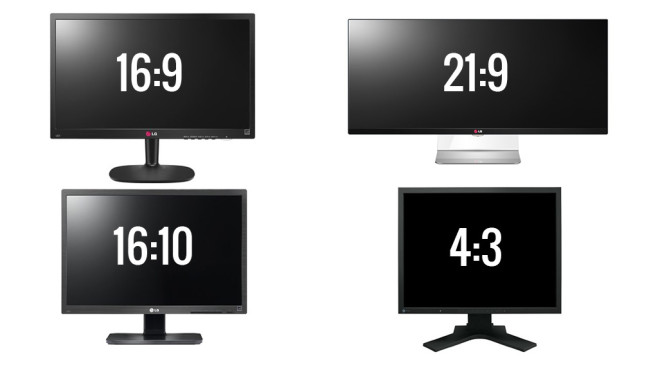
\includegraphics[height=5cm]{media/bs}
            \captionsetup{labelformat=empty}
            \caption{\color{red} Seitenverhältnis: das Verhältnis zwischen der Breite und der Höhe eines Bildes.}
            \label{fig:Seitenverhaeltnis}
        \end{figure}
        \begin{tabular}{|c|c|c|}
            \hline
            \textbf{Seitenverhältnis}   & \textbf{perfekt für}                                                   & \textbf{Welche Fernseher?}                                        \\ \hline
            {\color[HTML]{009901} 4:3}  & {\color[HTML]{CE6301} Alte Filme / Serien}                             & {\color[HTML]{3531FF} Alte Fernseher (häufig noch Röhrengeräte)}  \\ \hline
            {\color[HTML]{009901} 16:9} & {\color[HTML]{CE6301} Aktuelles Fernsehprogramm / Filme für Fernsehen} & {\color[HTML]{3531FF} Fast jeder moderne Flachbildfernseher}      \\ \hline
            {\color[HTML]{009901} 21:9} & {\color[HTML]{CE6301} Kinofilme}                                       & {\color[HTML]{3531FF} Wenige - meist Premium-Flachbildfernseher} \\ \hline
        \end{tabular}
    \end{center}

    \section{Softwarelizenzen}\label{sec:softwarelizenzen}

    \subsection{\color{red}Was sind Software-Lizenzen?}\label{subsec:was-sind-software-lizenzen?}

    \paragraph{Es handelt sich um eine rechtsverbindliche Vereinbarung zwischen Endnutzer und Softwarehersteller. Durch die Lizenz werden die Nutzungsbedingungen bis ins Detail geregelt. Die Lizenz ist also ein Vertrag, mit dem Urheber die Rechte an ihrem geistigen Eigentum auf andere überträgt. Dies geht immer mit einer direkten oder indirekten Gegenleistung einher, oder die Übertragung findet nur unter bestimmten Bedingungen statt}

    \subsection{\color{red}beschreibe, Lizenzmodelle und -arten mit wenigen Worten}\label{subsec:beschreibe-lizenzmodelle-und--arten-mit-wenigen-worten}
    \begin{center}
        \begin{tabular}{|l|l|}
            \hline
            \multicolumn{1}{|c|}{{\color[HTML]{00D2CB} Name der Lizenz}} & \multicolumn{1}{c|}{{\color[HTML]{00D2CB} Bedeutung}}                                         \\ \hline
            {\color[HTML]{CB0000} Freeware}                              & {\color[HTML]{3166FF} Kostenlose Nutzung, offene Sourcen}                                     \\ \hline
            {\color[HTML]{CB0000} Open Source}                           & {\color[HTML]{3166FF} Quellcode frei zugänglich, nicht immer kostenlos}                       \\ \hline
            {\color[HTML]{CB0000} Shareware}                             & {\color[HTML]{3166FF} Kostenlose Testung \& Verbreitung, meist beschränkte Version}           \\ \hline
            {\color[HTML]{CB0000} Donationware}                          & {\color[HTML]{3166FF} Spenden für Weiterentwicklung/ -betreibung}                             \\ \hline
            {\color[HTML]{CB0000} Standard Lizenz}                       & {\color[HTML]{3166FF} Entweder Gerät oder Account gebunden}                                   \\ \hline
            {\color[HTML]{CB0000} Abonnement basierte Lizenz}            & {\color[HTML]{3166FF} Kostenpflichtiges Abo, aber zeitlich beschränkt}                        \\ \hline
            {\color[HTML]{CB0000} EULA}                                  & {\color[HTML]{3166FF} Endbenutzerlizenzvertrag, festgelegte Nutzungsbedingungen}              \\ \hline
            {\color[HTML]{CB0000} Arbeitsstation Lizenz}                 & {\color[HTML]{3166FF} Nur für einen Computer, ein Back-Up meist erlaubt}                      \\ \hline
            {\color[HTML]{CB0000} Cloud basierte Lizenz}                 & {\color[HTML]{3166FF} Über Cloud jederzeit und überall zugreifbar}                            \\ \hline
            {\color[HTML]{CB0000} Aktivierungslizenz}                    & {\color[HTML]{3166FF} Lizenz zur Produktaktivierung}                                          \\ \hline
            {\color[HTML]{CB0000} Public Domain}                         & {\color[HTML]{3166FF} Kompletter Verzicht auf Urheberrechte, der Quellcode ist öffentlich}    \\ \hline
            {\color[HTML]{CB0000} Cardware}                              & {\color[HTML]{3166FF} Entwickler wünscht sich Postkarte von den Nutzern}                      \\ \hline
            {\color[HTML]{CB0000} Adware}                                & {\color[HTML]{3166FF} Software ist kostenlos, finanziert sich aber durch Werbung}             \\ \hline
            {\color[HTML]{CB0000} Kommerzielle Software-Lizenz}          & {\color[HTML]{3166FF} Nutzer erwirbt Nutzungsrechte an der Software, meist entgeltlich, kann} \\ \hline
            {\color[HTML]{CB0000} By Name}                               & {\color[HTML]{3166FF} auch gratis sein}                                                       \\ \hline
            {\color[HTML]{CB0000} No commercial use}                     & {\color[HTML]{3166FF} Kommerzielle Verwendung verboten}                                       \\ \hline
        \end{tabular}
    \end{center}

    \section{Green-IT}\label{sec:green-it}
    \subsection{\color{red}Ziele der Green-IT}\label{subsec:ziele-der-green-it}
        \begin{itemize}
            \color{magenta}
            \item Reduzierung des Energieverbrauchs
            \item Recyclings und Wiederverwendung
            von Geräten
            \item Nutzung erneuerbarer Energien
            \item Nachhaltigkeit von Unternehmen zu
            verbessern
            \item Langlebige Produkte herstellen
        \end{itemize}
    \subsection{\color{red}Erleuterung und Bennenug der Maßnahmen zur Reduzierung der Umweltbelastung}\label{subsec:erleuterung-und-bennenug-der-maßnahmen-zur-reduzierung-der-umweltbelastung}
        \begin{multicols}{2}
            \begin{enumerate}
                \color{magenta}
                \item Cloud-Hosting
                \begin{itemize}
                    \color{blue}
                    \item Reduziert den CO2-Ausstoß
                    \item Kostensenkung
                    \item weniger Geräte => weniger Energie verbraucht
                    \item Kunden verbrauchen 77\% weniger Server, 84\% weniger
                    Strom und reduzieren die Kohlenstoffemissionen um 88\%.
                \end{itemize}
                \color{magenta}
                \item Virtualisierung
                \begin{itemize}
                    \color{blue}
                    \item Senkung der Wartungskosten
                    \item Erhöhung der Sicherheit
                    \item Einfache Implementierung
                    \item Senkung der Energiekosten
                    \item Zentralisierte Verwaltung
                    \item Weniger Ausfallzeiten/höhere Produktivität
                \end{itemize}
                \color{magenta}
                \item REFURBISHING/RECYCLING
                \begin{itemize}
                    \color{blue}
                    \item Vermeidung von toxischer Verschmutzung
                    \item Vermeidet Elektroschrott
                \end{itemize}
                \color{magenta}
                \item Umweltschonende Hardware
                \begin{itemize}
                    \color{blue}
                    \item Kauf nur von nachhaltiger Hardware
                    \item Umweltfreundliche Labels
                    \item Verwendung von Hardware, die langlebiger ist
                \end{itemize}
                \color{magenta}
                \item Standby-Modus \& Geräte abschalten
                \begin{itemize}
                    \color{blue}
                    \item Konfiguration des Standby-Modus in allen Geräten
                    \item Unbenutzte Geräte ausschalten
                \end{itemize}
                \color{magenta}
                \item Nachhaltige Büros
                \begin{itemize}
                    \color{blue}
                    \item IT-Ausstattung dem individuellen Bedarf
                    anpassen
                    \item Papierloses Büro
                    \item Energiesparende Geräte kaufen
                    \item Mobile Arbeitsprozesse
                \end{itemize}
            \end{enumerate}
        \end{multicols}
    \subsection{\color{red}Umwelt-Prüfzeichen mit den grundlegenden Zielen}\label{subsec:umwelt-prüfzeichen-mit-den-grundlegenden-zielen}
        \begin{multicols}{2}
            \begin{figure}[H]
                \centering
                
\includegraphics[height=2cm]{media/estar}
                \captionsetup{labelformat=empty}
                \caption{\color{orange} Das Programm wurde 1992 von der US-
                Umweltschutzbehörde ins Leben gerufen,
                    wobei Computer und Monitore diese
                    Auszeichnung erhielten. Heutzutage findet
                    man das Zeichen auch auf Großgeräten,
                    Beleuchtungseinrichtungen und anderen
                    elektronischen Geräten.}
                \label{fig:estar}
            \end{figure}
            \begin{figure}[H]
                \centering
                
\includegraphics[height=2cm]{media/tco-certified}
                \captionsetup{labelformat=empty}
                \caption{\color{orange}Zeichnet Produkte wie Monitore,
                    Drucker oder Mobiltelefone aus, die
                    benutzer- und umweltfreundlich und
                    energieeffizient sind}
                \label{fig:tco}
            \end{figure}
            \begin{figure}[H]
                \centering
                
\includegraphics[height=2cm]{media/ECOLABEL}
                \captionsetup{labelformat=empty}
                \caption{\color{orange}Das Zeichen wird für Produkte und
                Dienstleistungen vergeben, die eine
                geringere Umweltbelastung aufweisen als
                vergleichbare Produkte. Das EU-
                Umweltzeichen soll den Verbrauchern die
                Möglichkeit geben, umweltfreundlichere und
                gesündere Produkte zu erkennen.}
                \label{fig:ECOLABEL}
            \end{figure}
            \begin{figure}[H]
                \centering
                
\includegraphics[height=2cm]{media/TUEV-Rheinland-Logo2.svg}
                \captionsetup{labelformat=empty}
                \caption{\color{orange}Das Zertifikat "Energieeffizientes
                Rechenzentrum" garantiert, dass sich das
                Unternehmen der Nachhaltigkeit verpflichtet
                fühlt.}
                \label{fig:TUEV}
            \end{figure}
        \end{multicols}
    
    \section{Netzteile und Kostenberechnung}\label{sec:netzteile-und-kostenberechnung}
        \subsection{\color{red}die Hauptfunktion von PC-Netzteilen}\label{subsec:die-hauptfunktion-von-pc-netzteilen}
        \paragraph{\color{codegreen} Das Computer-Netzteil wandelt den Wechselstrom (AC) 230 Volt aus einer Netzsteckdose in Niedervolt-Gleichstrom (DC) (3,3), (5) und (12) Volt zum Betrieb von Mainboard, Prozessor und Peripheriegeräten um.}
    \subsection{\color{red}den Stecker Main Power}\label{subsec:den-stecker-main-power}
        \begin{center}
            \begin{figure}[H]
                \centering
                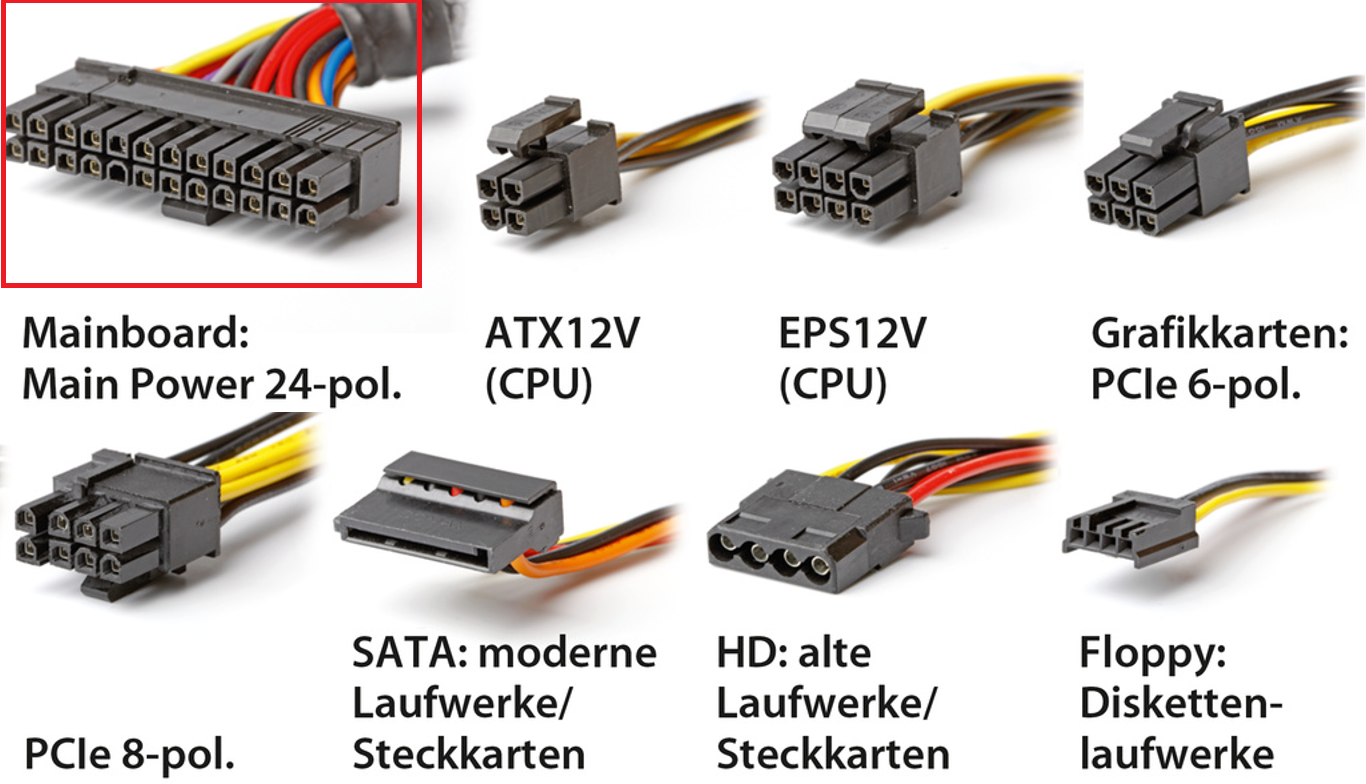
\includegraphics[height=5cm]{media/netzteile}
                \captionsetup{labelformat=empty}
                \caption{\color{orange} Main Power Stecker ist erste Stecker oben links }
                \label{fig:netzteile}
            \end{figure}
        \end{center}
    \subsection{\color{red}Erläuter die Bedeutung des 80-Plus-Zertifikates}\label{subsec:erläuter-die-bedeutung-des-80-plus-zertifikates}
        \paragraph{\color{codegreen} Das 80plus  ist eine initiative um Energie effizientere Netzteile besser vermarkten zu können und auch dementsprechend auszeichnen zu können.\color{blue}80 plus bedeutet, das Netzteil muss bei 20, 50
        und 100 Prozent last, mindestens einen Wirkungsgrad von 80 aufweisen.\color{codegreen}Das heißt weniger als oder maximal 20 prozent der aufgenommenen Energie darf quasi in Wärme umgewandelt. Es muss halt mindestens 80 Prozent der Hardware die am Netzteil angeschlossen ist dann auch zur Verfügung stehen.}
    \begin{center}
        \begin{figure}[H]
            \centering
            
\includegraphics[height=3cm]{media/80plus}
            \captionsetup{labelformat=empty}
            \caption{\color{orange} 80 PLUS ist eine nordamerikanische Initiative zur Förderung von PC-Netzteilen, die einen Wirkungsgrad von 80\% oder höher aufweisen. }
            \label{fig:80plus}
        \end{figure}
    \end{center}
    \subsection{\color{red}Berechnung der Energiekosten von elektrischen Geräten}\label{subsec:berechnung-der-energiekosten-von-elektrischen-geräten}
        \subsubsection{Beispiel: \color{white}\colorbox{red}{Sehr wichtig}}
            \paragraph{\color{codegreen} Im Rahmen des Umzugs sollen einige PCs neu angeschafft werden. Der Kunde soll sich zwischen Zwei PC-Varianten entscheiden. Beide PC-Varianten sind nahezu baugleich bis auf das verwendete Netzteil.}
            \paragraph{\color{codegreen}Sie wurden damit beauftragt, für eine Besprechung die Energieeffizienz der beide PCs unter ökonomischen Gesichtspunkten zu vergleichen}
            \paragraph{\color{red}Betriebsstunden:}
            \begin{itemize}
                \item \colorbox{yellow}{9 Stunden pro Tag}
                \item Betrieb an \colorbox{yellow}{20 Arbeitstagen pro Monat}
            \end{itemize}
            \paragraph{\color{red}Die beiden zu vergleichen Pcs sind wie folgt ausgestattet:}
            \begin{itemize}
                \color{magenta}
                \item PC-A hat ein niedrigpreisiges Netzteil ohne Zertifikat.
                \item PC-B hat ein Netzteil nach dem 80Plus Gold Standard.
            \end{itemize}
            \paragraph{\colorbox{yellow}{Errechnen} Sie die \colorbox{yellow}{Leistung} und die \colorbox{yellow}{Energiekosten} pro Monat, wenn eine \colorbox{yellow}{kWh 30 Cent} kostet.}
            \paragraph{\color{codegreen} Dem englischsprachigen Manual des Netzteils können Sie folgende Definition entnehmen:}
            \paragraph{\color{codegreen} Efficiency = Useful power output/Total power input}
            \begin{center}
                \begin{tabular}{|c|c|c|}
                    \hline
                    & {\color[HTML]{32CB00} PC-A} & {\color[HTML]{32CB00} PC-B \color[HTML]{FFD700}(80 Plus Gold)} \\ \hline
                    {\color[HTML]{32CB00} Wirkungsgrad des Netztei ls bei 60 W in \%} & {\color[HTML]{32CB00} 43\%}    & {\color[HTML]{32CB00} 76\%} \\ \hline
                    {\color[HTML]{32CB00} Durchschnittl iche Leistung im Betrieb}    & {\color[HTML]{32CB00} 60 W}     & {\color[HTML]{32CB00} 60 W}  \\ \hline
                    {\color[HTML]{32CB00} Bezogene Leistung aus Stromnetz}           & {\color[HTML]{32CB00} 139,53 W} & {\color[HTML]{FE0000} ?}    \\ \hline
                    {\color[HTML]{32CB00} Energiekosten pro Monat in €}              & {\color[HTML]{CB0000} ?}       & {\color[HTML]{FE0000} ?}    \\ \hline
                \end{tabular}
            \end{center}

    \subsubsection{\color{white} \colorbox{codegreen}{Lösung}}
    \paragraph{\color{codegreen} - Energiekosten pro Monat in € bei PC-A}
    \begin{equation*}
        Stunden\:pro\:Monat=Stunden\:pro\:Tag\times Arbeitstagen\:pro\:Monat
    \end{equation*}
    \begin{equation*}
        =>9\:\times 20\:=\:\colorbox{yellow}{180\: h}
    \end{equation*}
    \begin{equation*}
        Monatlich\:Bezogene\:Leistung\:in\:\left(Wh\right)\:=\:Bezogene\:Leistung\:aus\:Stromnetz\:\left(W\right)\:\times Stunden\:pro\:Monat\:\left(h\right)
    \end{equation*}
    \begin{equation*}
        =>  139,53\:W\:\times \:180\:h\:=\colorbox{yellow}{25115,4 Wh}
    \end{equation*}
    \begin{equation*}
        Monatlich\:Bezogene\:Leistung\:in\:\left(kWh\right)\:=\:\frac{25115,4 Wh}{1000}=\colorbox{yellow}{25,11 kWh}
    \end{equation*}
    \begin{equation*}
        Energiekosten\:pro\:Monat\:in\:€\:=Monatlich\:Bezogene\:Leistung\:\times \:1\: kWh\:kosten
    \end{equation*}
    \begin{equation*}
        => 25,11\:kWh\:\times \:0,3\:€\:=\:\colorbox{yellow}{7,53 €}
    \end{equation*}
    \begin{center}
        \begin{tabular}{|c|c|c|}
            \hline
            & {\color[HTML]{32CB00} PC-A} & {\color[HTML]{32CB00} PC-B \color[HTML]{FFD700}(80 Plus Gold)} \\ \hline
            {\color[HTML]{32CB00} Wirkungsgrad des Netztei ls bei 60W in \%} & {\color[HTML]{32CB00} 43\%}    & {\color[HTML]{32CB00} 76\%} \\ \hline
            {\color[HTML]{32CB00} Durchschnittl iche Leistung im Betrieb}    & {\color[HTML]{32CB00} 60 W}     & {\color[HTML]{32CB00} 60 W}  \\ \hline
            {\color[HTML]{32CB00} Bezogene Leistung aus Stromnetz}           & {\color[HTML]{32CB00} 139,53 W} & {\color[HTML]{FE0000} ?}    \\ \hline
            {\color[HTML]{32CB00} Energiekosten pro Monat in €}              & {\color[HTML]{CB0000} \colorbox{yellow}{7,53 €}}       & {\color[HTML]{FE0000} ?}    \\ \hline
        \end{tabular}
    \end{center}
    \paragraph{\color{codegreen} - Bezogene Leistung aus Stromnetz PC-B}
    \begin{equation*}
        Bezogene\:Leistung\:aus\:Stromnetz\:=\:\frac{Durchschnittliche\:Leistung\:im\:Betrieb}{Wirkungsgrad\:des\:Netzteils}\cdot 100
    \end{equation*}
    \begin{equation*}
        =>\frac{60\:W}{76\:}\cdot 100\:=\colorbox{yellow}{78.94 W}
    \end{equation*}
    \begin{center}
        \begin{tabular}{|c|c|c|}
            \hline
            & {\color[HTML]{32CB00} PC-A} & {\color[HTML]{32CB00} PC-B \color[HTML]{FFD700}(80 Plus Gold)} \\ \hline
            {\color[HTML]{32CB00} Wirkungsgrad des Netztei ls bei 60 W in \%} & {\color[HTML]{32CB00} 43\%}    & {\color[HTML]{32CB00} 76\%} \\ \hline
            {\color[HTML]{32CB00} Durchschnittl iche Leistung im Betrieb}    & {\color[HTML]{32CB00} 60 W}     & {\color[HTML]{32CB00} 60 W}  \\ \hline
            {\color[HTML]{32CB00} Bezogene Leistung aus Stromnetz}           & {\color[HTML]{32CB00} 139,53 W} & {\color[HTML]{FE0000} \colorbox{yellow}{78,94 W}}    \\ \hline
            {\color[HTML]{32CB00} Energiekosten pro Monat in €}              & {\color[HTML]{CB0000} 7,53 €}       & {\color[HTML]{FE0000} ?}    \\ \hline
        \end{tabular}
    \end{center}
    \paragraph{\color{codegreen} - Energiekosten pro Monat in € bei PC-B}
    \begin{equation*}
        Monatlich\:Bezogene\:Leistung\:in\:\left(Wh\right)\:=\:Bezogene\:Leistung\:aus\:Stromnetz\:\left(W\right)\:\times Stunden\:pro\:Monat\:\left(h\right)
    \end{equation*}
    \begin{equation*}
        =>  78,94\:W\:\times \:180\:h\:=\colorbox{yellow}{14209,2 Wh}
    \end{equation*}
    \begin{equation*}
        Monatlich\:Bezogene\:Leistung\:in\:\left(kWh\right)\:=\:\frac{14209,2\:Wh}{1000}=\colorbox{yellow}{14,2 kWh}
    \end{equation*}
    \begin{equation*}
        Energiekosten\:pro\:Monat\:in\:€\:=Monatlich\:Bezogene\:Leistung\:\times \:1\:kWh\:kosten
    \end{equation*}
    \begin{equation*}
        => 14,2\:kWh\:\times \:0,3\:€\:=\:\colorbox{yellow}{4,26 €}
    \end{equation*}
    \begin{center}
        \begin{tabular}{|c|c|c|}
            \hline
            & {\color[HTML]{32CB00} PC-A} & {\color[HTML]{32CB00} PC-B \color[HTML]{FFD700}(80 Plus Gold)} \\ \hline
            {\color[HTML]{32CB00} Wirkungsgrad des Netztei ls bei 60W in \%} & {\color[HTML]{32CB00} 43\%}    & {\color[HTML]{32CB00} 76\%} \\ \hline
            {\color[HTML]{32CB00} Durchschnittl iche Leistung im Betrieb}    & {\color[HTML]{32CB00} 60 W}     & {\color[HTML]{32CB00} 60 W}  \\ \hline
            {\color[HTML]{32CB00} Bezogene Leistung aus Stromnetz}           & {\color[HTML]{32CB00} 139,53 W} & {\color[HTML]{FE0000} 78,94 W}    \\ \hline
            {\color[HTML]{32CB00} Energiekosten pro Monat in €}              & {\color[HTML]{CB0000} 7,53 €}       & {\color[HTML]{FE0000} \colorbox{yellow}{4,26 €}}    \\ \hline
        \end{tabular}
    \end{center}

    \section{Tastatur und Maus}\label{sec:tastatur-und-maus}
    \subsection{\color{red} Was sind die Unterschiede zwischen einer mechanischen und der Rubberdome-Tastatur}\label{subsec:was-sind-die-unterschiede-zwischen-einer-mechanischen-und-der-rubberdome-tastatur}
    \begin{multicols}{2}
        \subsubsection{\color{codegreen} Rubber-Dome-Tastatur}
        \begin{itemize}
            \color{blue}
            \item Eine Rubberdome Tastatur ist meist etwas leiser als eine mechanische.
            \item Man kann drei, maximal sechs Tasten gleichzeitig drücken, sodass diese alle vom Gerät registriert werden.
            \item schafft im Durchschnitt rund fünf Millionen Anschläge
        \end{itemize}
        \subsubsection{\color{codegreen} Mechanische Tastaturen}
        \begin{itemize}
            \color{blue}
            \item Mechanische Tastaturen sind etwas robuster und schwerer als Rubberdome
            \item mechanische Tastatur ermöglicht das Drücken und Registrieren aller Tasten gleichzeitig.
            \item überlebt 50 bis 70 Millionen Anschläge
        \end{itemize}
    \end{multicols}
    \subsection{\color{red}Beschreibe die Unterschiede zwischen einer mechanisch-linearen und mechanisch-taktilen Tastatur}\label{subsec:beschreibe-die-unterschiede-zwischen-einer-mechanisch-linearen-und-mechanisch-taktilen-tastatur}
    \subsubsection{\color{codegreen}Linearer Schalter}
    \paragraph{\color{codegreen}Sie fühlen sich vom Moment, an dem man eine Taste zu drücken beginnt, bis zu dem Moment, an dem man
    die Taste vollständig durchgedrückt hat, stets gleich an. Es gibt kein taktiles oder akustisches Feedback um einen
    erfolgreichen Tastendruck zu bestätigen, folglich werden die Tasten die meiste Zeit voll angeschlagen}
    \paragraph{\color{codegreen} Andre Beschreibung:\\\color{red}Ein Spürbarer Wiederstand\\\color{codegreen} Der taktile Switch reagiert am Schaltpunkt mit einem leichten, sehr präzisen und sofortigen Feedback. Ideal für Gaming Turniere und FPS-Gaming}
    \subsubsection{\color{codegreen}Taktiler  Schalter}
    \paragraph{\color{codegreen}liefern ein taktiles Feedback wenn der Umschalt- oder Klickpunkt erreicht wurden. Beim Drücken einer Taste
    spürt man also einen kleinen Widerstand und weiß somit, dass der Tastendruck erfolgreich registriert wurde.}
    \paragraph{\color{codegreen} Andre Beschreibung\\\color{red} Reibungsloser, fließender Tastenanschlag\\\color{codegreen} Die fließenden Funktionsweise linearer Switches eignet sich besonders für doppelte und schnelle mehrfache Anschläge. Sie sind ideal für Action-Spiele}
    \begin{center}
        \begin{figure}[H]
            \centering
            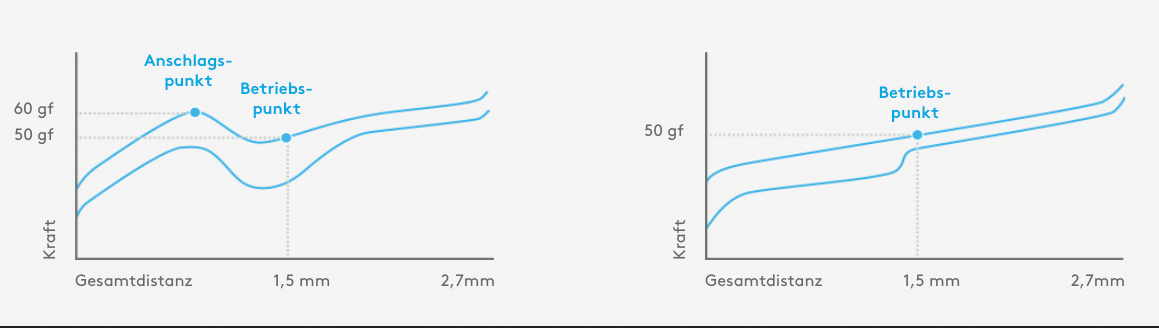
\includegraphics[height=3cm]{media/tactile_vs_linear}
            \captionsetup{labelformat=empty}
            \caption{\color{orange} tactile vs linear. Tactile links \& Linear rechts}
            \label{fig:tactile_vs_kinear}
        \end{figure}
    \end{center}
    \subsection{\color{red}Erläutere die Unterschiede zwischen einer mechanischen, einer optischen und einer Laser-Maus}\label{subsec:erleutere-die-unterschiede-zwischen-einer-mechanischen-einer-optischen-und-einer-laser-maus}
    \begin{center}
        \begin{tabular}{|c|l|}
            \hline
            {\color[HTML]{9A0000} Art der Maus}     & {\color[HTML]{9A0000} Mechanismus}                                                                          \\ \hline
            {\color[HTML]{3166FF} } &
                {\color[HTML]{009901} \begin{tabular}[c]{@{}l@{}}- Eine kleine Kugel wird im Inneren gehalten und berührt das Pad durch ein Loch\\  an der Unterseite der Maus.\end{tabular}} \\
            {\color[HTML]{3166FF} Mechanische Maus} & {\color[HTML]{009901} - Wenn die Maus bewegt wird, rollt der Ball}                                          \\
            {\color[HTML]{3166FF} }                 & {\color[HTML]{009901} - Diese Bewegung des Balls wird in Signale umgewandelt und an den Computer gesendet.} \\ \hline
            {\color[HTML]{3166FF} }                 & {\color[HTML]{009901} - Misst die Bewegung und Beschleunigung des Zeigers}                                  \\
            {\color[HTML]{3166FF} Optische Maus} &
                {\color[HTML]{009901} - Es verwendet eine Lichtquelle anstelle einer Kugel, um die Bewegung des Zeigers zu beurteilen} \\
            {\color[HTML]{3166FF} }                 & {\color[HTML]{009901} - Die optische Maus ist weniger oberflächenempfindlich}                               \\ \hline
            {\color[HTML]{3166FF} }                 & {\color[HTML]{009901} - Misst die Bewegung und Beschleunigung des Zeigers}                                  \\
            {\color[HTML]{3166FF} Laser-Maus}       & {\color[HTML]{009901} - Laser Mouse verwendet Laserlicht}                                                   \\
            {\color[HTML]{3166FF} }                 & {\color[HTML]{009901} - Laser Mouse ist hochempfindlich und kann auf jeder harten Oberfläche arbeiten}      \\ \hline
        \end{tabular}
    \end{center}
    \subsection{\color{red} Beschreibe den Begriff Trackball}\label{subsec:beschreibe-den-begriff-trackball}
    \paragraph{\color{codegreen} Trackball: Der Trackball ähnelt dem umgedrehten Design der Maus. Der Benutzer bewegt den Ball direkt, während das Gerät selbst stationär bleibt. Der Benutzer dreht den Ball in verschiedene Richtungen, um durch die Bildschirmbewegungen zu navigieren.}
    
    \section{Drucker}\label{sec:drucker}
    \subsection{\color{red} Vor-und Nachteile von Tintenstrahldruckern, Laserdruckern und Matrixdruckern}\label{subsec:vor-und-nachteile-von-tintenstrahldruckern-laserdruckern-und-matrixdruckern}
    \subsubsection{\color{codegreen}Tintenstrahldruckern}
    \begin{itemize}
        \color{red}
        \item Vorteile
        \begin{itemize}
            \color{blue}
            \item Hohe Druckqualität auf gutem Papier
            \item Foto ähnlicher Druck auf Spezialpapier
            \item Geringe Umweltbelastung
            \item Günstige Druckerpreise
            \item leise beim Druck
        \end{itemize}
        \item Nachteile
        \begin{itemize}
            \color{blue}
            \item Hohe Materialkosten
            \item normaleweise Nicht wasserfest
            \item Niedrige Geschwindigkeit bei hoher Qualität
            \item Verfließende Tinte auf saugfähigen Papier
            \item kann der Druckkopf bei Tintendruckern austrocknen, wenn sie länger nicht benutzt werden.
        \end{itemize}
    \end{itemize}
    \subsubsection{\color{codegreen}Laserdruckern}
    \begin{itemize}
        \color{red}
        \item Vorteile
        \begin{itemize}
            \color{blue}
            \item Hohe Druckqualität
            \item Hohe Seitenleistung
            \item Geringe Druckkosten
            \item Geringe Umweltbelastung
            \item Hohe Zuverlässigkeit
            \item Lange Lebensdauer
        \end{itemize}
        \item Nachteile
        \begin{itemize}
            \color{blue}
            \item hohe Anschaffungskosten
            \item Farblaser sind noch sehr teuer und sperrig
            \item Keine Fotoqualität beim Ausdruck möglich
        \end{itemize}
    \end{itemize}
    \subsubsection{\color{codegreen}Matrixdruckern}
    \begin{itemize}
        \color{red}
        \item Vorteile
        \begin{itemize}
            \color{blue}
            \item Günstiger Druck
            \item Durchschläge möglich
            \item Geringe Umweltbelastung
            \item Druck auf Endlospapier
            \item Drucken mit Durchschlägen möglich
            \item Wartungsarm und geringe Verbrauchskosten
            \item Das einzige Verbrauchsmaterial ist das Farbband
        \end{itemize}
        \item Nachteile
        \begin{itemize}
            \color{blue}
            \item sehr laut
            \item nur bedingt grafikfähig
            \item ungeeignet für Farbdruck
            \item langsamer Druck
            \item können nicht alle Zeichen und Grafiken gedruckt
            \item können keine Folien bedruckt werden
            \item aufgrund der geringen Fertigungszahlen ist  der Anschaffungspreis mittlerweile sehr hoch für Nadeldrucker
        \end{itemize}
    \end{itemize}
    \subsection{\color{red} Beschreibe die grundlegende Funktionsweise der drei oben genannten Druckertypen}\label{subsec:beschreibe-die-grundlegende-funktionsweise-der-drei-oben-genannten-druckertypen}
    \subsubsection{\color{codegreen}Tintenstrahldrucker}
    \paragraph{\color{codegreen}Das Drucker- bzw. Fotopapier  wird durch einen präzisen Schrittmotor durch den Drucker geschoben. Dabei fährt der Druckkopf über das Druckmedium und beschießt es mit einer Vielzahl winziger Tintentröpfchen oder einem durchgehenden Tintenstrahl.}
    \subsubsection{\color{codegreen}Laserdrucker}
    \paragraph{\color{codegreen}Bei Beginn des Druckvorganges wird die im Drucker vorhandene Bildtrommel über einen Koronadraht elektrostatisch negativ geladen. Mit einer Laserdiode und einem Spiegel werden nun die Teile der Trommel mit Laserlicht belichtet, welche später den Toner tragen sollen. Anschließend wird die Bildtrommel, an der sogenannten Entwicklereinheit vorbeigeführt. Diese Entwicklereinheit enthält den Toner. Dieser ist negativ geladen und haftet somit an den durch den Laser neutralisierten Stellen auf der Bildtrommel. Nach der Austragung des Toners dreht sich die Bildtrommel weiter und überträgt den Toner auf das positiv geladene Papier. Da die Tonerpartikel nur schwach gebunden auf dem Papier haften, müssen sie anschließend dauerhaft mit dem Papier verbunden werden. Dazu passiert das Papier die sogenannte Fixiereinheit. Dabei handelt es sich im Normalfall um zwei Walzen. Einer dieser Walzen ist hohl und enthält einen Heizdraht, welcher die Walze auf etwa 180 Grad Celsius aufheizt. Durch die Hitze und den Druck der Walze wird der Toner dauerhaft mit dem Papier verbunden und dieses verlässt anschließend den Drucker.}
    \subsubsection{\color{codegreen}Matrixdruckern}
    \paragraph{\color{codegreen} Bei einem Nadeldrucker wird ein mit Tinte getränktes oder mit Kohlenstoff beschichtetes Farbband an einem Druckkopf vorbeigezogen, während Nadeln die Punkte auf das Papier hämmern. Die vertikale Anzahl der Nadeln bestimmt die Auflösung des Druckers, es gibt von 7 bis 48 Nadeln zahlreiche Varianten, wobei ein 24-Nadel-Drucker technisch 360 dpi Auflösung erreichen kann.}
    


    \section{Anschlüsse am Mainboard}\label{sec:anschlüsse-am-mainboard}
    \subsection{\color{red} Benenne die verschiedenen Anschlüsse eines Mainboards und erläutere deren Einsatzzwecke}\label{subsec:benenne-und-erläuter-den-einsatzzwecke-von-der-verschiedenen-anschlüsse-eines-mainboards}
    \begin{center}
        \begin{figure}[H]
            \centering
            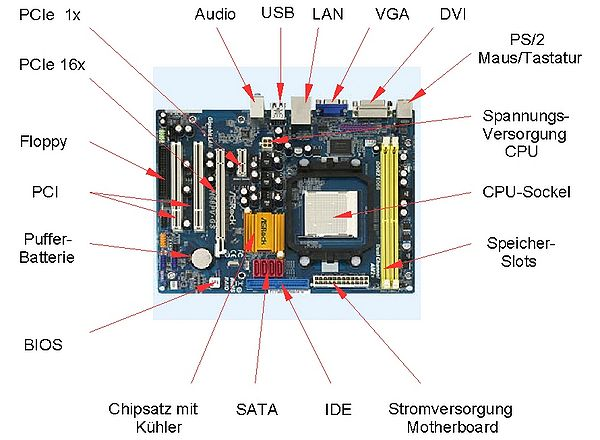
\includegraphics[height=10cm]{media/Motherboard}
            \captionsetup{labelformat=empty}
            \caption{Hauptplatine}
            \label{fig:Motherboard}
        \end{figure}
    \end{center}
    \subsubsection{\color{codegreen}PCIe}
    \paragraph{\color{codegreen}Peripheral Component Interconnect Express (PCIe) ist eine schnelle interne Schnittstelle für Erweiterungskarten in Computer-Systemen. Mit der Einführung von PCIe im Jahr 2004 wurde dem AGP als Grafikkarten-Schnittstelle ein Ende gesetzt und auch der PCI als internes Computer-Bussystem abgelöst.}
    \begin{center}
        \begin{figure}[H]
            \centering
            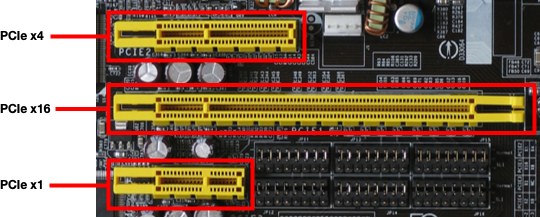
\includegraphics[height=3cm]{media/pcie}
            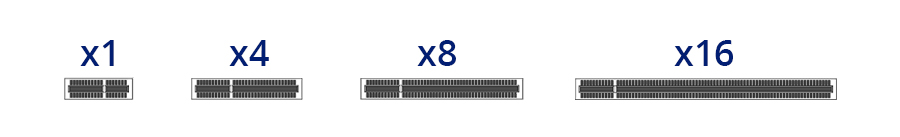
\includegraphics[height=2cm]{media/pci2}
            \captionsetup{labelformat=empty}
            \caption{Vergleich verschiedener PCIe-Kartengrößen }
            \label{fig:pcie}
        \end{figure}
    \end{center}
    \subsubsection{\color{codegreen}VGA-Port}
    \paragraph{\color{codegreen}VGA-Anschluss (engl. Video Graphics Array) umfasst die Spezifikation einer analogen elektronischen Schnittstelle zur Übertragung von Bewegtbildern zwischen Grafikkarten und Anzeigegeräten sowie Spezifikationen für hierzu geeignete Stecker und Kabel.}
    \begin{center}
        \begin{figure}[H]
            \centering
            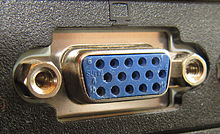
\includegraphics[height=3cm]{media/VGA}
            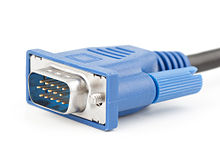
\includegraphics[height=3cm]{media/VGA-cable}
            \captionsetup{labelformat=empty}
            \caption{VGA Port und Stecker}
            \label{fig:VGA}
        \end{figure}
    \end{center}
    \subsubsection{\color{codegreen}DVI-Port}
    \paragraph{\color{codegreen}DVI (Digital Video Interface) ist eine Schnittstelle für die digitale und analoge Übertragung von Videodaten. Sie gilt als digitaler Nachfolger des S-VGA-Standards und hat sich über viele Jahre neben HDMI als Verbindung zwischen Computern und Monitoren etabliert.}
    \begin{center}
        \begin{figure}[H]
            \centering
            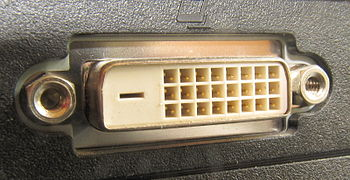
\includegraphics[height=3cm]{media/dvi}
            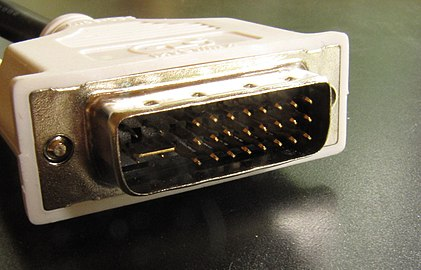
\includegraphics[height=3cm]{media/DVI-Stecker}
            \captionsetup{labelformat=empty}
            \caption{DVI Port und Stecker}
            \label{fig:dvi}
        \end{figure}
    \end{center}
    \subsubsection{\color{codegreen}HDMI}
    \paragraph{\color{codegreen}HDMI ist eine Schnittstelle zur Übertragung von hochauflösenden, digitalen Video- und Audio-Daten. HDMI verbindet Abspielgeräte, wie Computer oder Video-Player mit einem Display oder Beamer. HDMI baut auf DVI auf. Somit ist HDMI zu DVI abwärtskompatibel.}
    \begin{center}
        \begin{figure}[H]
            \centering
            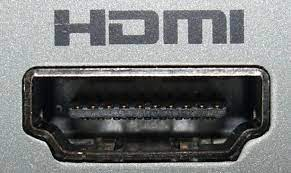
\includegraphics[height=3cm]{media/hdmi}
            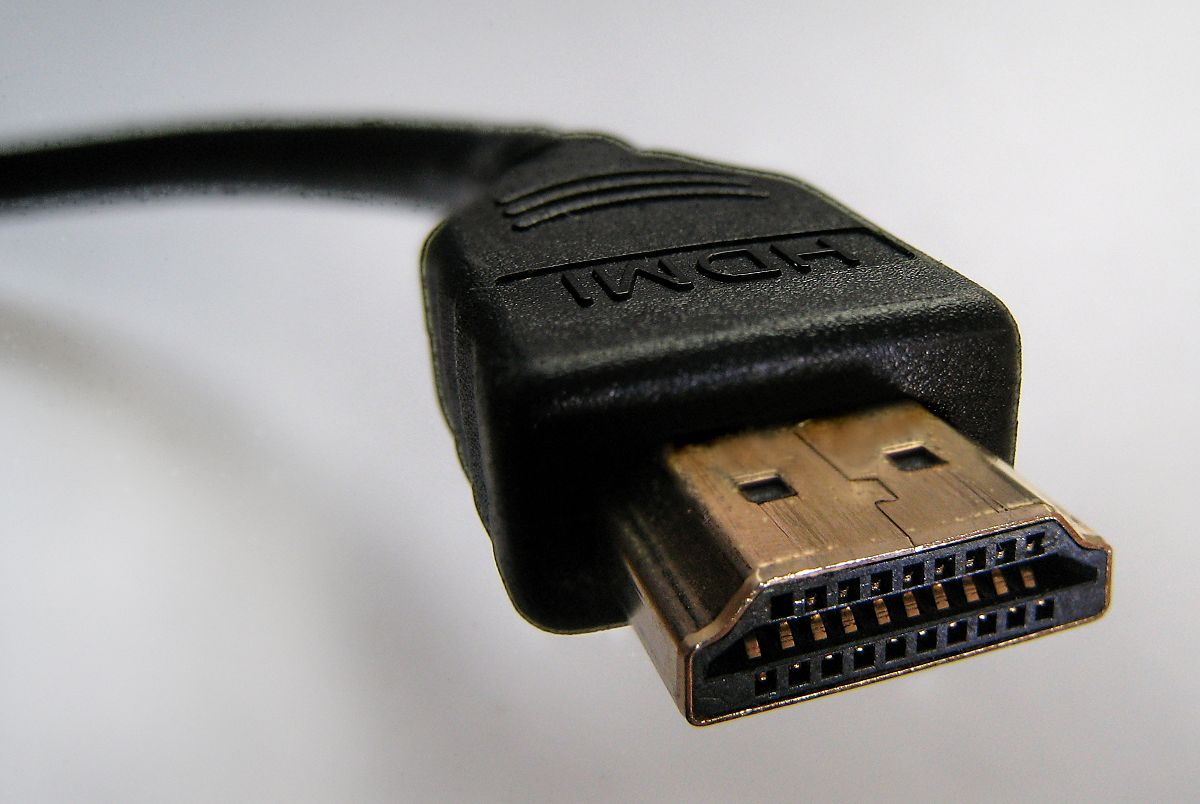
\includegraphics[height=3cm]{media/hdmikable}
            \captionsetup{labelformat=empty}
            \caption{HDMI Port und Kable}
            \label{fig:hdmi}
        \end{figure}
    \end{center}
    \subsubsection{\color{codegreen}Chipsatz}
    \paragraph{\color{codegreen}Ein Chipsatz besteht aus mehreren Schaltkreisen, die zusammen eine Einheit bilden. Der Chipsatz funktioniert als Verbindungsglied zwischen den einzelnen Komponenten eines Computers. Das heißt der Chipsatz verbindet CPU mit RAM, ROM und allen anderen Komponenten, Schnittstellen und Bausätzen.}
    \subsubsection{\color{codegreen}CPU-Sockel}
    \paragraph{\color{codegreen}Auf dem sogenannten Prozessorsockel wird die CPU (Central Processing Unit), der Hauptprozessor, angebracht.}
    \subsubsection{\color{codegreen}RAM-Steckplätze}
    \paragraph{\color{codegreen}Steckplätze für den RAM (Random Access Memory), den Arbeitsspeicher, gibt es in der Regel zwei bis vier.}
    \subsubsection{\color{codegreen}BIOS-Chip}
    \paragraph{\color{codegreen}Das BIOS (Basic Input/Output System) führt bei jedem Start des Computers einen System-Check durch und initialisiert alle angeschlossenen Hardware-Komponenten.}
    \subsubsection{\color{codegreen}SATA-Anschlüsse}
    \paragraph{\color{codegreen}Bei einem SATA-Anschluss (Serial Advanced Attachement) handelt es sich um einen Standard für die Datenübertragung, der die älteren IDE-Anschlüsse aufgrund einer besseren Datentransferrate abgelöst hat. An die SATA-Anschlüsse werden Festplatten (HDD oder SSD) und optische Laufwerke angeschlossen.}

    \section{Festplatten}\label{sec:festplatten}
    \subsection{\color{red} Erläutere die Funktionsweise einer HDD und einer SSD}\label{subsec:erläutere-die-funktionsweise-einer-hdd-und-einer-ssd}
    \subsubsection{\color{codegreen} HDD}
    \paragraph{\color{codegreen}Eine Festplatte ist ein Massenspeicher, bei dem die Daten magnetisch gespeichert werden. Im Inneren einer Festplatte befinden sich deshalb eine oder mehrere magnetisierbare Scheiben, die auf einer Spindel gestapelt sind und rotieren. Ähnlich einem Plattenspieler wandern mehrere Schreib-/Leseköpfe über den Magnetscheiben von außen nach innen und zurück. Sie schreiben Informationen, indem sie die Plattenoberfläche magnetisieren, und lesen Informationen, indem sie die Magnetisierung abtasten.}
    \subsubsection{\color{codegreen}SSD}
    \paragraph{\color{codegreen}Die Speicherung auf einer SSD wird über Halbleiter realisiert, ähnlich der Speicherbausteine für den Arbeitsspeicher. Die Speichermethode entspricht der, die Sie von Speicherkarten oder USB-Stick kennen. Im Gegensatz zur HDD besitzt eine SSD keinen Lese- und Schreibkopf und auch sonst keine mechanisch beweglichen Teile. Dadurch ist der Zugriff auf Daten deutlich schneller.}

    \begin{center}
        \begin{figure}[H]
            \centering
            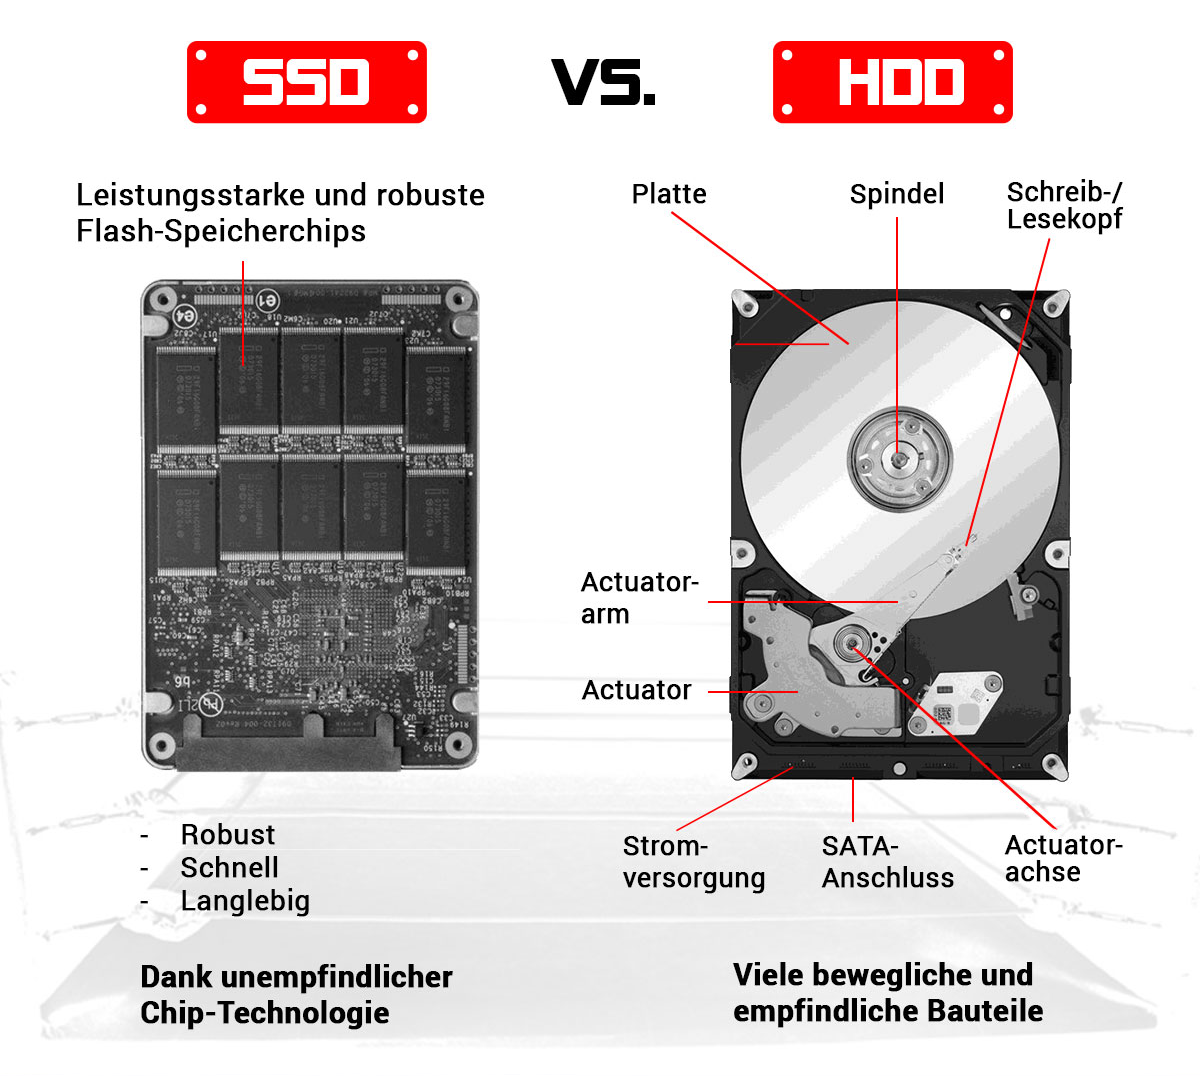
\includegraphics[height=6cm]{media/hddsdd}
            \captionsetup{labelformat=empty}
            \caption{HDD vs SSD}
            \label{fig:hddsdd}
        \end{figure}
    \end{center}
    \subsection{\color{red}Benenne Vor- und Nachteile zwischen einer SSD und einer HDD}\label{subsec:bennenne-vor--und-nachteile-zwischen-einer-ssd-und-einer-hdd}
    \begin{center}
        \begin{tabular}{|l|l|l|}
            \hline
            {\color[HTML]{3531FF} } &
                {\color[HTML]{3531FF} SSD} &
                {\color[HTML]{3531FF} HDD} \\ \hline
            {\color[HTML]{009901} Vorteile} &
                {\color[HTML]{009901} \begin{tabular}[c]{@{}l@{}}- in der Regel schnellste Transferraten\\ - geringste Zugriffszeiten\\ - wsentlich geringerer Stromverbrauch\\ - stoßfest\\ - lautloser Betrieb\\ - geringes Gewicht und kompaktere Maße (SATA-SSDs\end{tabular}} &
                {\color[HTML]{009901} \begin{tabular}[c]{@{}l@{}}- höchste Speicherkapazität\\ -langlebiger als SSDs\\ -sehr günstiger Preis\end{tabular}} \\ \hline
            {\color[HTML]{9A0000} Nachteile} &
                {\color[HTML]{9A0000} \begin{tabular}[c]{@{}l@{}}- immer noch viel teurer als HHD\\ - begrenzte Speicherkapazität\\ - begrenze Anzahl an Schreibvorgängen je Speicherzelle\end{tabular}} &
                {\color[HTML]{9A0000} \begin{tabular}[c]{@{}l@{}}- langsamer als SSDs und SSDHs\\ - höhere Zugriffzeiten \\ - höherer Stromverbrauch\\ - anfällig gegen Erschütterungen \\ - höheres Gewicht\\ - lauter Betrieb\end{tabular}} \\ \hline
        \end{tabular}
    \end{center}
    \subsection{\color{red} Beschreibe den Aufbau einer SSHD}\label{subsec:bescreibe-den-aufbau-einer-sshd}

    \paragraph{\color{codegreen}Solid-State Hybrid Drives, kurz SSHDs, sind Hybrid-Festplatten, die aus einer herkömmlichen Festplatte mit einem zusätzlichen Flash-Speicher bestehen. Der Flash-Speicher dient als Datenpuffer für Schreib- und Lesezugriffe und soll für kürzere Zugriffszeiten sorgen.}

    \section{RAID und NAS}\label{sec:raid-und-nas}
    \subsection{\color{red}Beschreibe die Funktionsweise von RAID 0, 1 und 5 und deren Vor- und Nachteile}\label{subsec:beschreibe-die-funktionsweise-von-raid-0-1-und-5}
    \subsubsection{\color{codegreen}RAID 0}
    \paragraph{\color{codegreen}Bei einem RAID 0 werden mindestens 2 Festplatten benötigt. Die Daten werden dabei auf mehrere Festplatten verteilt, wenn eine Festplatte ausfällt, wären alle Daten verloren. Ein RAID 0 ist ein Verfahren ohne irgendeinen Schutz vor Verlust, da aber von beiden Festplatten gleichzeitig gelesen werden kann, ist die Lese- und Schreibgeschwindigkeit sehr hoch. Die Nutzungskapazität der verfügbaren Laufwerke beträgt 100\%.\\}
    \begin{vwcol}[widths={0.6,0.4}]
        \begin{tabular}{ll}
            \multicolumn{2}{c}{RAID 0}                                                  \\ \hline
            \multicolumn{1}{l|}{Technik}            & Streifen                          \\
            \multicolumn{1}{l|}{Vorteil}            & Extrem schnell                    \\
            \multicolumn{1}{l|}{Nachteil}           & Keine Ausfallsicherheit von Daten \\
            \multicolumn{1}{l|}{Anwendungsbeispiel} & Laufwerk für Datenbankserver
        \end{tabular}
        \begin{figure}[H]
            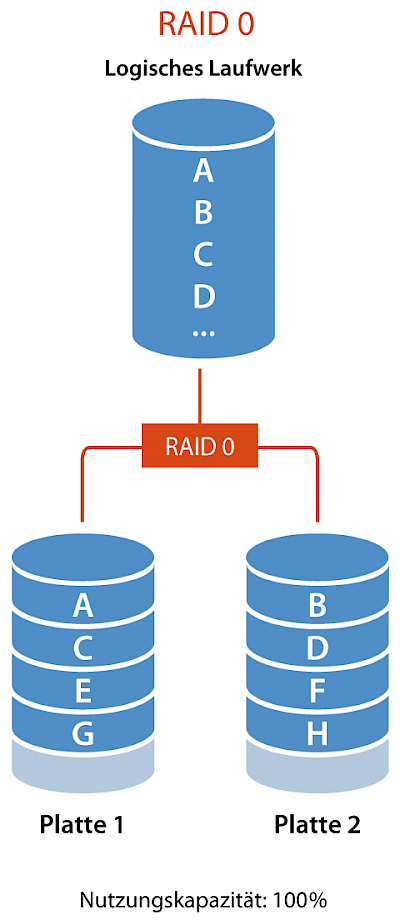
\includegraphics[height=4cm]{media/raid0}
            \label{fig:raid0}
        \end{figure}
    \end{vwcol}

    \subsubsection{\color{codegreen}RAID 1}
    \paragraph{\color{codegreen}Bei einem RAID 1 werden mindestens 2 Festplatten benötigt. Dieselben Daten werden dabei auf beiden Festplatten gespeichert. Dies hat Vor- und Nachteile: Einerseits sind die Daten noch vorhanden, wenn eine Festplatte ausfallen würde, andererseits braucht man die doppelte Anzahl Festplatten, weil die effektive Speicherkapazität halbiert wird. Die Nutzungskapazität der verfügbaren Laufwerke beträgt daher 50\%.\\}
        \begin{vwcol}[widths={0.6,0.4}]
            \begin{tabular}{ll}
                \multicolumn{2}{c}{RAID 1}                                                \\ \hline
                \multicolumn{1}{l|}{Technik}            & Spiegelung                      \\
                \multicolumn{1}{l|}{Vorteil}            & Schnell mit Ausfallsicherheit   \\
                \multicolumn{1}{l|}{Nachteil}           & Tiefe Nutzungskapazität         \\
                \multicolumn{1}{l|}{Anwendungsbeispiel} & Laufwerk für das Betriebssystem
            \end{tabular}
            \begin{figure}[H]
                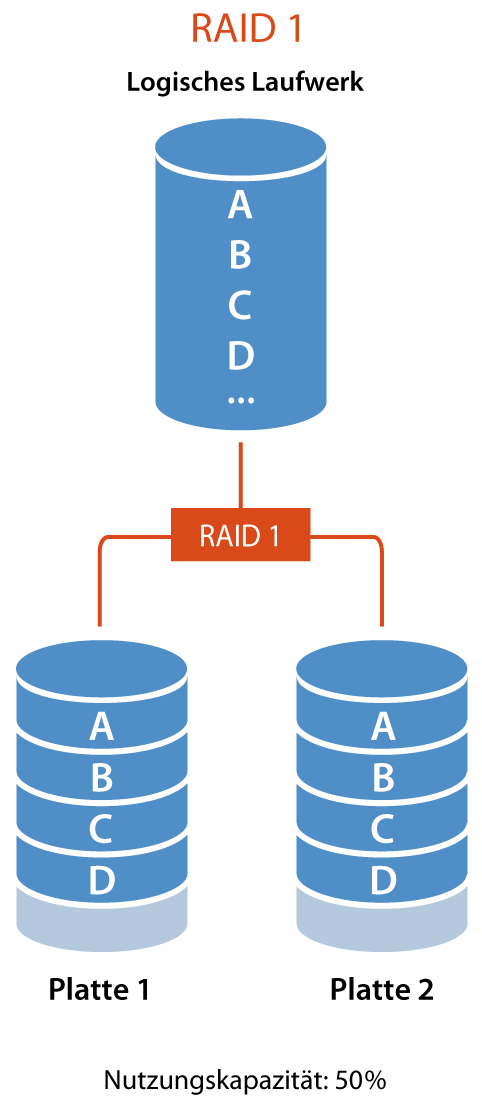
\includegraphics[height=4cm]{media/raid1}
                \label{fig:raid1}
            \end{figure}
        \end{vwcol}
    \subsubsection{\color{codegreen}RAID 5}
    \paragraph{\color{codegreen}Bei einem RAID 5 benötigt man mindestens 3 Festplatten. Die Daten werden auf alle Festplatten verteilt. Zusätzlich wird ein Paritätswert errechnet und gespeichert. Wenn eine Festplatte ausfallen sollte, kann der RAID-Kontroller anhand dieser Parität die fehlenden Daten errechnen. Dieses Verfahren benötigt zwar eine Festplatte weniger als ein entsprechendes RAID 1 System, es muss aber für alle Daten eine Paritätswert berechnet werden, was mehr Rechenleistung benötigt. Ein RAID 5-System kann aus maximal 16 Festplatten bestehen. Die Nutzungskapazität der im RAID 5 verfügbaren Laufwerke beträgt 67\% - 94\% (Gesamtkapazität minus 1 Laufwerk).\\}
    \begin{vwcol}[widths={0.6,0.4}]
        \begin{tabular}{ll}
            \multicolumn{2}{c}{RAID 5}                                                \\ \hline
            \multicolumn{1}{l|}{Technik}            & Streifen mit Parität            \\
            \multicolumn{1}{l|}{Vorteil}            & Ausfallsicherheit               \\
            \multicolumn{1}{l|}{Nachteil}           & Langsame Schreibgeschwindigkeit \\
            \multicolumn{1}{l|}{Anwendungsbeispiel} & Laufwerke für Archivsysteme
        \end{tabular}
        \begin{figure}[H]
            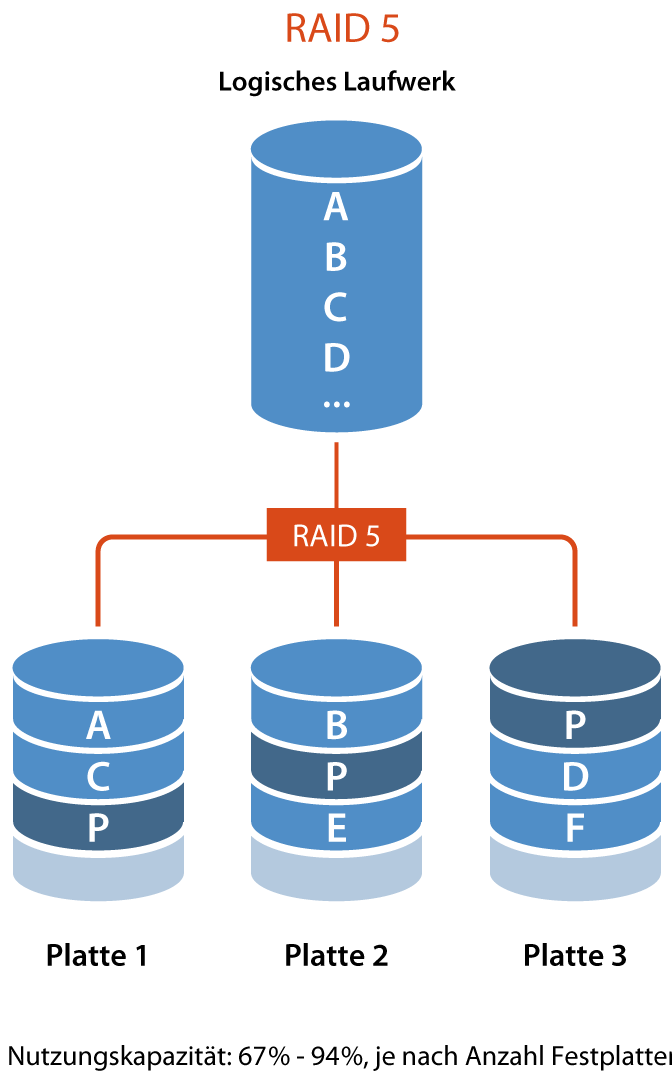
\includegraphics[height=4cm]{media/raid5}
            \label{fig:raid5}
        \end{figure}
    \end{vwcol}
    \subsection{\color{red} Erläutere den Nutzen von einem NAS}\label{subsec:erläutere-den-nutzen-von-einem-nas}
    \paragraph{\color{codegreen}NAS ermöglicht es Anwendern, effektiver zusammenzuarbeiten und Daten gemeinsam zu nutzen, insbesondere Arbeitsteams, die sich an entfernten Standorten oder in verschiedenen Zeitzonen befinden. Ein NAS stellt eine Verbindung zu einem drahtlosen Router her, so dass in verteilten Arbeitsumgebungen der Zugriff auf Dateien und Ordner von jedem mit dem Netzwerk verbundenen Gerät aus problemlos möglich ist. Unternehmen setzen in der Regel eine NAS-Umgebung als Grundlage für eine Private Cloud ein.}
    \section{Cloud-Computing, ERP, Smart-Factory}\label{sec:cloud-computing-erp-smart-factory}
    \subsection{\color{red} Beschreibe die Unterschiede zwischen Private-Cloud und Public-Cloud}\label{subsec:beschreibe-die-unterschiede-zwischen-private-cloud-und-public-cloud}
    \paragraph{\color{codegreen}Eine Private Cloud ist ein Cloud-Service, der nicht mit einer anderen Organisation gemeinsam genutzt wird. Die Nutzer einer Private Cloud haben diese Cloud für sich.
    Im Unterschied dazu ist eine Public Cloud ein Cloud-Service, bei dem Computing-Dienste von verschiedenen Kunden gemeinsam genutzt werden. Die in der Cloud befindlichen Daten und Anwendungen der einzelnen Kunden sind jedoch für die anderen Cloud-Kunden nicht sichtbar.}
    \begin{center}
        \begin{figure}[H]
            \centering
            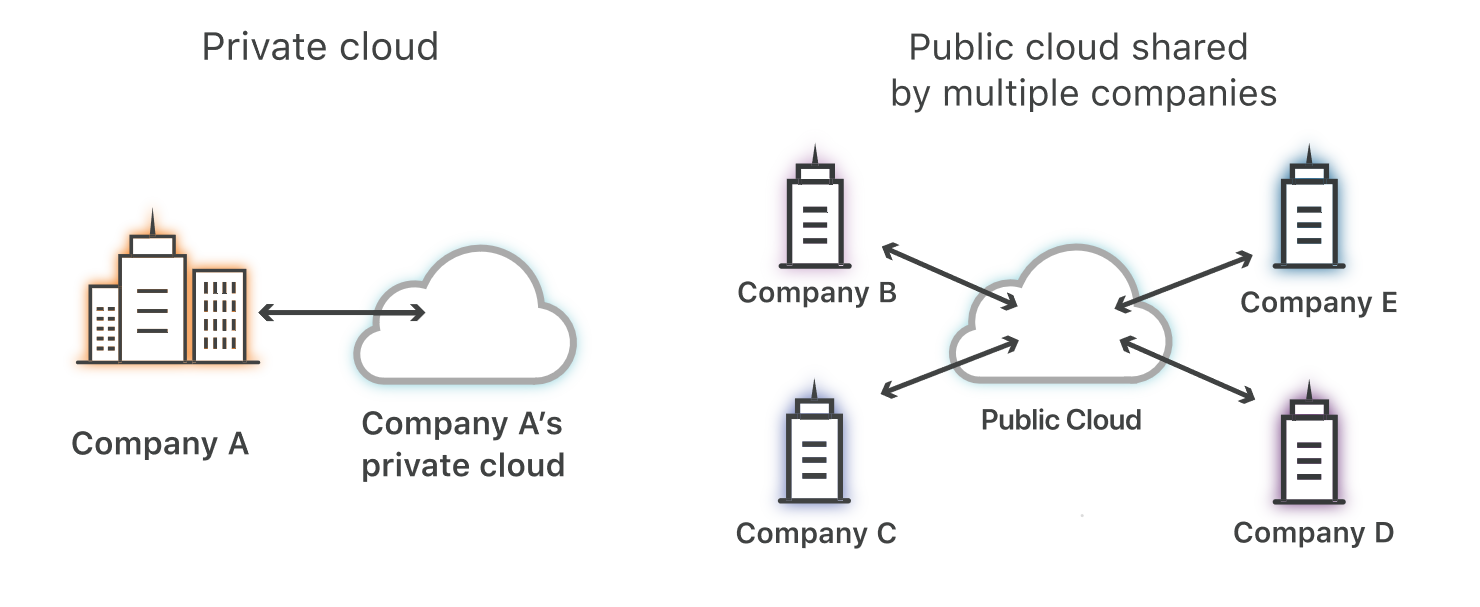
\includegraphics[height=5cm]{media/cloud}\label{fig:cloud}
        \end{figure}
    \end{center}
    \subsection{\color{red}Beschreibe Cloud-Computing-Systeme (IaaS, PaaS, SaaS)}\label{subsec:beschreibe-cloud-computing-systeme-(iaas-paas-saas)}
    \subsubsection{\color{codegreen}Infrastructure as a Service (IaaS)}
    \paragraph{\color{codegreen}Ein Provider bietet Kunden Zugang zu Speicher, Netzwerkkomponenten, Servern und weiteren IT-Ressourcen in der Cloud, die auf der Basis der Nutzung abgerechnet werden.\\\color{red}z.B.
    Google Cloud Dienste}
    \subsubsection{\color{codegreen}Platform as a Service (PaaS)}
    \paragraph{\color{codegreen}Ein Service-Provider bietet den Nutzern Zugang zu einer Cloud-basierten Umgebung, in der sie Anwendungen entwickeln und bereitstellen können. Der Provider stellt die zugrunde liegende Infrastruktur zur Verfügung.\\\color{red}z.B.
    Microsoft Azure, Amazon Web Services (AWS)}
    \subsubsection{\color{codegreen}Software as a Service (SaaS)}
    \paragraph{\color{codegreen}Ein Service-Provider stellt Software und Anwendungen über das Internet bereit. Die Nutzer „abonnieren“ die Software und greifen per Web oder über APIs des Anbieters darauf zu.\\
    \color{red}z.B. (Office 365), Github}
    \subsection{\color{red}Erkläre die fünf ERP-Managementbereiche}\label{subsec:erkläre-die-fünf-erp-managementbereiche}
    \subsubsection{\color{codegreen}Human Resource Management HRM}
    \paragraph{\color{codegreen}bezeichnet die Organisation und Verwaltung des Personals in einem Unternehmen und ist mit dem deutschen Begriff Personalmanagement gleichzusetzen.}
    \subsubsection{\color{codegreen}Customer Relationship Management CRM}
    \paragraph{\color{codegreen}also Kundenbeziehungsmanagement, bezeichnet eine Strategie zur systematischen Gestaltung der Beziehungen und Interaktionen einer Organisation mit bestehenden und potenziellen Kunden.}
    \subsubsection{\color{codegreen}Material Requirements Planning MRP}
    \paragraph{\color{codegreen}Die Materialbedarfsplanung ist ein System zur Berechnung der Materialien und Komponenten, die zur Herstellung eines Produkts benötigt werden.}
    \subsubsection{\color{codegreen}Supply Chain Management SCM}
    \paragraph{\color{codegreen} bezeichnet den Aufbau und die Verwaltung integrierter Logistikketten (Material- und Informationsflüsse) über den gesamten Wertschöpfungsprozess, ausgehend von der Rohstoffgewinnung über die Veredelungsstufen bis hin zum Endverbraucher.}
    \subsubsection{\color{codegreen}Financial Resource Management FRM}
    \paragraph{\color{codegreen}Finanzmanagement bedeutet Planung, Organisation, Leitung und Kontrolle der finanziellen Aktivitäten wie Beschaffung und Verwendung von Mitteln des Unternehmens. Es bedeutet die Anwendung allgemeiner Managementprinzipien auf die finanziellen Ressourcen des Unternehmens.}
    \subsection{\color{red} Erkläre den Begriff SMART-Factory anhand eines Beispiels}\label{subsec:erkläre-den-begriff-smart-factory-anhand-eines-beispiels}
    \paragraph{\color{codegreen}SmartFactory bedeutet eine voll datenintegrierte und „ intelligente “ Fabrik . Die Zielstellung wird als Industrie 4.0 bezeichnet. Auf jeder Stufe der Datenannahme , Datenverarbeitung und Datenweitergabe sollen „ intelligente “ Softwarelösungen die Flexibilität und Effizienz der Produktion sicherstellen , Vorhersagen erstellen und Produktionspläne optimieren . Damit soll die Fabrik transparent ständig alle Informationen bereitstellen.\\\color{red} Beispiele:}
    \begin{itemize}
        \color{magenta}
        \item Maschinen , Lager- und Transportsysteme mit ihren Steuerungen , Prüfmitteln und der Betriebstechnik sind vollständig in ihren Datensystemen vernetzt.
        \item Sensoren dienen zur Erfassung von Qualitäts- und Prozessdaten.
        \item Aktoren steuern physisch Maschinen und Anlagen.
        \item Die Onlineverbindung zu Kunden , Lieferanten und Geschäftspartnern hält alle Prozessbeteiligten laufend informiert.
    \end{itemize}
    \begin{center}
        \color{red}\Huge Done!
    \end{center}
\end{document}